\documentclass[acmsmall,screen,review]{acmart} 
% Note: Removed 'anonymous' option based on TALLIP usually being Single-Blind. 
% CHECK THE SUBMISSION PORTAL: If it says "Double-Blind", add 'anonymous' back.

\usepackage{grffile}
\usepackage{fontspec}
\usepackage{tabularx}
\usepackage{multirow}
\usepackage{booktabs}
\usepackage{xltabular}
\usepackage{array}
\usepackage[section]{placeins}

% Ensure the .ttf is in the same folder for compilation
\newfontfamily\bengalifont[Script=Bengali]{NotoSansBengali-Regular.ttf}
\newcommand{\bn}[1]{{\bengalifont #1}}

%% Journal metadata
\acmJournal{TALLIP}
\acmYear{2025}
\setcopyright{acmcopyright}
\copyrightyear{2025}

%% Reference Style
\bibliographystyle{ACM-Reference-Format}

\begin{document}

%% 1. TITLE REVISION
%% Guidelines: "Typically, a title contains from 6 to 12 words."
%% Your original title was 18 words.
%% Suggested Short Title:
\title{Optimizing Bengali Semantic Retrieval: Monolingual vs. Multilingual Embeddings with Matryoshka Learning}

%% 2. AUTHOR SECTION
%% Guidelines: "Authors' names should be given... along with affiliated organizations."
%% NOTE: TALLIP is typically Single-Blind (Reviewers know you, you don't know them).
%% Unless the submission portal explicitly says "Double-Blind", you should UNCOMMENT your names.

\author{Koshik Debanath}
\email{koshik.debanath@gmail.com}
\affiliation{%
  \institution{Rajshahi University of Engineering and Technology}
  \country{Bangladesh}
}

\author{Azmain Yakin Srizon}
\email{azmainsrizon@gmail.com}
\affiliation{%
  \institution{Rajshahi University of Engineering and Technology}
  \country{Bangladesh}
}

\renewcommand{\shortauthors}{Debanath and Srizon}

%% 3. ABSTRACT REVISION
%% Guidelines: "Avoid the use of the first person." (No "We", "Our")
%% Guidelines: "150 to 200 words."
\begin{abstract}
Effective semantic retrieval remains the primary bottleneck for Bengali Retrieval-Augmented Generation (RAG) systems. While general-purpose multilingual models exist, they often lack the specific semantic alignment required for high-precision tasks. This paper conducts a comparative study of three distinct embedding architectures—monolingual (\texttt{shihab17}), distilled multilingual (\texttt{distiluse}), and paraphrase-focused (\texttt{mpnet})—to identify the optimal foundation for Bengali retrieval. These models are fine-tuned on the BanglaRQA dataset using a composite objective of Multiple Negatives Ranking Loss and Matryoshka Representation Learning (MRL). The results demonstrate that architectural choice is decisive: the fine-tuned \texttt{mpnet} model achieves a superior NDCG@10 of \textbf{0.8114}, statistically outperforming the monolingual baseline. Beyond raw performance, deployment constraints typical of low-resource environments are addressed. An efficiency analysis reveals that high-dimensional vectors are largely redundant for this task; the MRL-trained MPNet model retains \textbf{96\%} of its retrieval effectiveness at just \textbf{128 dimensions}, offering an 83\% reduction in storage costs without compromising accuracy. Code and fine-tuned models are released to facilitate reproducibility and further research at: \url{https://github.com/kowshik24/Bangla-Embedding}
\end{abstract}

%% CCS Concepts (Required)
\begin{CCSXML}
<ccs2012>
   <concept>
       <concept_id>10010147.10010178.10010179</concept_id>
       <concept_desc>Computing methodologies~Natural language processing</concept_desc>
       <concept_significance>500</concept_significance>
   </concept>
   <concept>
       <concept_id>10002951.10003317.10003338</concept_id>
       <concept_desc>Information systems~Retrieval models and ranking</concept_desc>
       <concept_significance>500</concept_significance>
   </concept>
   <concept>
       <concept_id>10010147.10010257.10010293.10010294</concept_id>
       <concept_desc>Computing methodologies~Neural networks</concept_desc>
       <concept_significance>300</concept_significance>
   </concept>
 </ccs2012>
\end{CCSXML}

\ccsdesc[500]{Computing methodologies~Natural language processing}
\ccsdesc[500]{Information systems~Retrieval models and ranking}
\ccsdesc[300]{Computing methodologies~Neural networks}

%% Keywords (Required)
\keywords{Bengali Language, Sentence Embeddings, Fine-Tuning, Information Retrieval, Matryoshka Representation Learning, RAG}

\maketitle


\section{Introduction}

Large Language Models (LLMs) have demonstrated transformative capabilities across a spectrum of natural language tasks. However, their practical deployment is often hampered by two critical weaknesses: a tendency to "hallucinate" facts not present in their training data and an inability to access timely or proprietary information. Retrieval-Augmented Generation (RAG) has emerged as the dominant architectural paradigm to address these shortcomings \cite{lewis2020retrieval, gao2023survey}. By dynamically retrieving relevant context from an external knowledge base before generation, RAG systems ground LLM outputs in factual reality, significantly mitigating hallucinations and enhancing their utility.

The efficacy of any RAG system, however, hinges critically on its retrieval component, which is typically powered by dense vector embeddings. While this technology is mature for high-resource languages like English, it remains a significant bottleneck for the vast majority of the world's languages. This challenge is particularly acute for Bengali, a language spoken by over 300 million people. Despite its large speaker base, Bengali is considered a "low-resource" language in the context of deep learning, suffering from a scarcity of curated datasets, commercially incentivized models, and research focus compared to English. Consequently, the choice of an embedding model is often driven by availability rather than empirical performance.

While multilingual models like XLM-RoBERTa \cite{conneau2019unsupervised} provide a strong foundation, they are often generalists that lack the specific semantic alignment required for question-answering tasks. Conversely, monolingual models may capture linguistic nuances but lack the architectural robustness of larger multilingual checkpoints. This dichotomy presents a research gap: identifying which architecture yields the highest fidelity for Bengali semantic retrieval when subjected to specialized fine-tuning.

This paper addresses this gap through a comprehensive study. We select three diverse architectures: a dedicated Bengali transformer, a lightweight distilled multilingual model, and a robust MPNet-based model. We subject all three to an identical fine-tuning regimen on the BanglaRQA dataset \cite{ekram2022banglarqa}, employing Matryoshka Representation Learning (MRL) \cite{kusupati2022matryoshka} to enforce efficiency. Our contributions are threefold. First, we provide a comparative benchmark of these architectures, demonstrating that while all benefit from fine-tuning, the architectural priors of the \texttt{mpnet} model offer superior ceiling performance. Second, we validate the effectiveness of MRL through extensive saturation and retention analysis. Third, we perform a qualitative analysis of downstream RAG performance, correlating retrieval metrics with generation faithfulness.

\section{Related Work}

\subsection{Retrieval-Augmented Generation (RAG)}
The core concept of augmenting generation with external knowledge, pioneered by \cite{lewis2020retrieval}, has evolved into a complex and rapidly advancing subfield of NLP. The academic discourse has broadly categorized its evolution into distinct phases. Early implementations, often referred to as "Naive RAG," employed a straightforward retrieve-then-read pipeline where a user query directly drives a semantic search, and the top-k retrieved documents are concatenated into the LLM's context window. While effective, this approach is susceptible to issues like misaligned retrieval and context overload \cite{hu2024comprehensive}.

Recent literature details a shift towards "Advanced RAG," which incorporates sophisticated pre- and post-retrieval strategies. These include query transformations (e.g., query rewriting, expansion), advanced indexing techniques (e.g., multi-vector retrieval), and re-ranking mechanisms to refine retrieved results before generation \cite{gao2023survey}. The current state-of-the-art is moving towards "Modular RAG," where the pipeline is deconstructed into interconnected modules that can be dynamically orchestrated based on query complexity, showcasing the field's progression towards more robust and adaptive systems. Our work focuses on the foundational retrieval module, as its optimization is a prerequisite for the success of any advanced RAG strategy, particularly in non-English contexts.

\subsection{Semantic Search in Low-Resource Languages}
While multilingual models offer a zero-shot baseline for many languages, their performance in specialized retrieval tasks for low-resource languages is often suboptimal. This performance gap stems from several factors, including inefficient tokenization of morphologically rich languages, semantic drift where word meanings are biased towards high-resource training data, and a lack of cultural and domain-specific context \cite{lin2024improving}. Recent work has begun to tackle these challenges directly within the Bengali language ecosystem. For example, \cite{debanath2025advancing} explored fine-tuning a generative model, Llama, for Bengali question-answering, establishing new benchmarks. However, such generative approaches are fundamentally dependent on the quality of retrieved context. An inaccurate or irrelevant context will invariably lead to a poor or hallucinated response, regardless of the generator's quality.

This dependency underscores the criticality of a robust retrieval component. Addressing this challenge has become a critical area of research. For instance, \cite{lin2024improving} demonstrates that fine-tuning multilingual models on even small, curated datasets in the target language can yield substantial performance gains. Other innovative approaches aim to overcome data scarcity through novel training paradigms. A notable example is Retrieval-Augmented Retrieval (RAR) \cite{yasunaga2022retrieval}, which uses a generate-then-retrieve cycle to synthesize training data, a technique that holds promise for languages where labeled pairs are scarce. Our study contributes to this area by providing a rigorous empirical benchmark that quantifies the impact of task-specific fine-tuning on diverse model architectures for Bengali, offering a clear pathway for practitioners to move beyond unreliable zero-shot baselines.

\subsection{Bengali Information Processing}
Recent research in \textit{ACM Transactions on Asian and Low-Resource Language Information Processing (TALLIP)} highlights the growing focus on specialized modeling for Bengali. For instance, Ghosal et al. demonstrated the efficacy of text embedding models combined with fuzzy SVMs for detecting hate speech in Bengali social media content \cite{ghosal2023inculcating}. Similarly, Chowdhury et al. analyzed the impact of transcription errors on Bengali spoken document summarization, emphasizing the need for robust semantic representations that can withstand noisy inputs \cite{chowdhury2024analyzing}. In the specific domain of retrieval, Das et al. introduced \textit{Anwesha}, a prototype for semantic search in Bangla that leverages WordNet and LSA \cite{das2022anwesha}. Shi et al. further explored cross-lingual transfer for document retrieval, showing that training on English data can benefit low-resource languages like Bengali \cite{shi2021crosslingual}. Our work extends this lineage by focusing specifically on the optimization of dense vector spaces for Question Answering, a critical component for RAG systems that has yet to be fully benchmarked for Bengali.


\subsection{Matryoshka and Efficient Embeddings}
Matryoshka Representation Learning (MRL) has recently gained traction as a standard for flexible embedding deployment. The release of \texttt{jina-embeddings-v3} demonstrated that MRL can be effectively scaled to multilingual contexts using Task LoRA adapters \cite{sturua2024jina}. Furthermore, recent frameworks like Matryoshka-Adaptor \cite{yoon2024matryoshka} and Quantization Aware Matryoshka Adaptation (QAMA) \cite{ahemad2025quantization} have shown that it is possible to reduce dimensionality and precision simultaneously while retaining over 95\% of retrieval performance. Our study applies these cutting-edge efficiency techniques to the specific morphological and semantic challenges of the Bengali language.

\subsection{Advancements in Sentence Embeddings for Bengali}
The Bengali NLP landscape has matured significantly with the development of foundational models. Early efforts produced models like BanglaBERT \cite{bhattacharjee2020banglabert}, which was pre-trained on a large Bengali corpus using a Masked Language Modeling (MLM) objective. While powerful for natural language understanding tasks, the pooling of raw token embeddings from such models is not inherently optimized for semantic similarity tasks. This limitation spurred the development of dedicated sentence-transformer models.

The advent of bi-encoder architectures, popularized by Sentence-BERT (SBERT) \cite{reimers2019sentence}, marked a paradigm shift. This methodology has been actively adopted for Bengali, with a common strategy being cross-lingual knowledge distillation from powerful English teacher models. For instance, the \texttt{shihab17/bangla-sentence-transformer} used in our study was developed by fine-tuning an XLM-RoBERTa student model on machine-translated datasets, using a multilingual SBERT model as the teacher \cite{uddin2024bangla}. Similarly, the BanglaEmbed models were created using a comparable distillation technique to produce lightweight and efficient sentence encoders \cite{kabir2024banglaembed}. Our work builds directly upon this foundation. By applying a unified, task-specific fine-tuning regimen to these and other architectures, we aim to move beyond the initial pre-training and isolate the impact of the base model's architectural priors on final retrieval performance for a demanding question-answering task.

\subsection{Efficient Representation Learning}
As vector databases grow to billions of entries, the dimensionality of embeddings becomes a critical factor for storage costs, memory usage, and query latency. Matryoshka Representation Learning (MRL) \cite{kusupati2022matryoshka} offers a principled solution to this challenge.

Formally, MRL reframes representation learning as a multi-scale optimization problem. The central idea is to learn a high-dimensional embedding vector, $z \in \mathbb{R}^d$, such that its prefixes are also effective, lower-dimensional representations. To achieve this, MRL defines a set of nested "Matryoshka" dimensions, $M \subset \{1, \dots, d\}$, typically chosen by halving the dimensionality (e.g., $M = \{d, d/2, d/4, \dots, 64\}$). The model, parameterized by $\theta_F$, learns a function $F(\cdot; \theta_F)$ that maps an input $x$ to the embedding $z$.

The key innovation lies in modifying the training objective. Instead of calculating the loss only on the final $d$-dimensional embedding, MRL computes and aggregates the loss at each of the chosen granularities $m \in M$. For a given training objective $\mathcal{L}_{\text{task}}$, such as the Multiple Negatives Ranking Loss used in our work, the MRL objective for a single data point $(x_i, y_i)$ is formulated as a weighted sum over the nested dimensions:
\begin{equation}
\min_{\theta_F, \{W^{(m)}\}_{m \in M}} \frac{1}{N} \sum_{i=1}^{N} \sum_{m \in M} c_m \cdot \mathcal{L}_{\text{task}}\left(W^{(m)} \cdot F(x_i; \theta_F)_{1:m}, y_i\right)
\end{equation}
Here, $F(x_i; \theta_F)_{1:m}$ denotes the output embedding truncated to its first $m$ dimensions, $W^{(m)}$ is a task-specific classification head for that dimension, and $c_m$ are scaling coefficients (typically set to 1). By optimizing this composite loss, the model is explicitly forced to encode the most critical semantic information into the initial dimensions of the embedding vector, with finer details layered into subsequent dimensions.

This approach stands in contrast to traditional dimensionality reduction techniques such as Principal Component Analysis (PCA) or autoencoders, which require a separate, post-hoc training step and can result in significant information loss. MRL's primary advantage is that it integrates efficiency directly into the training objective, enabling flexible, on-the-fly truncation at inference time. An application can use the full 768-dimensional vector for high-precision tasks and a truncated 128-dimensional prefix for low-latency lookups, all from a single learned representation. Our study is the first to systematically apply and evaluate MRL for the Bengali language, demonstrating its viability for creating highly efficient yet powerful retrieval systems.

% \newpage

\section{Methodology}

Our experimental framework involves fine-tuning three distinct base models using a unified training strategy to ensure a fair comparison. See the figure \ref{fig:architecture}.

\begin{figure}[H]
    \centering
    % Placeholder for your Architecture Diagram
    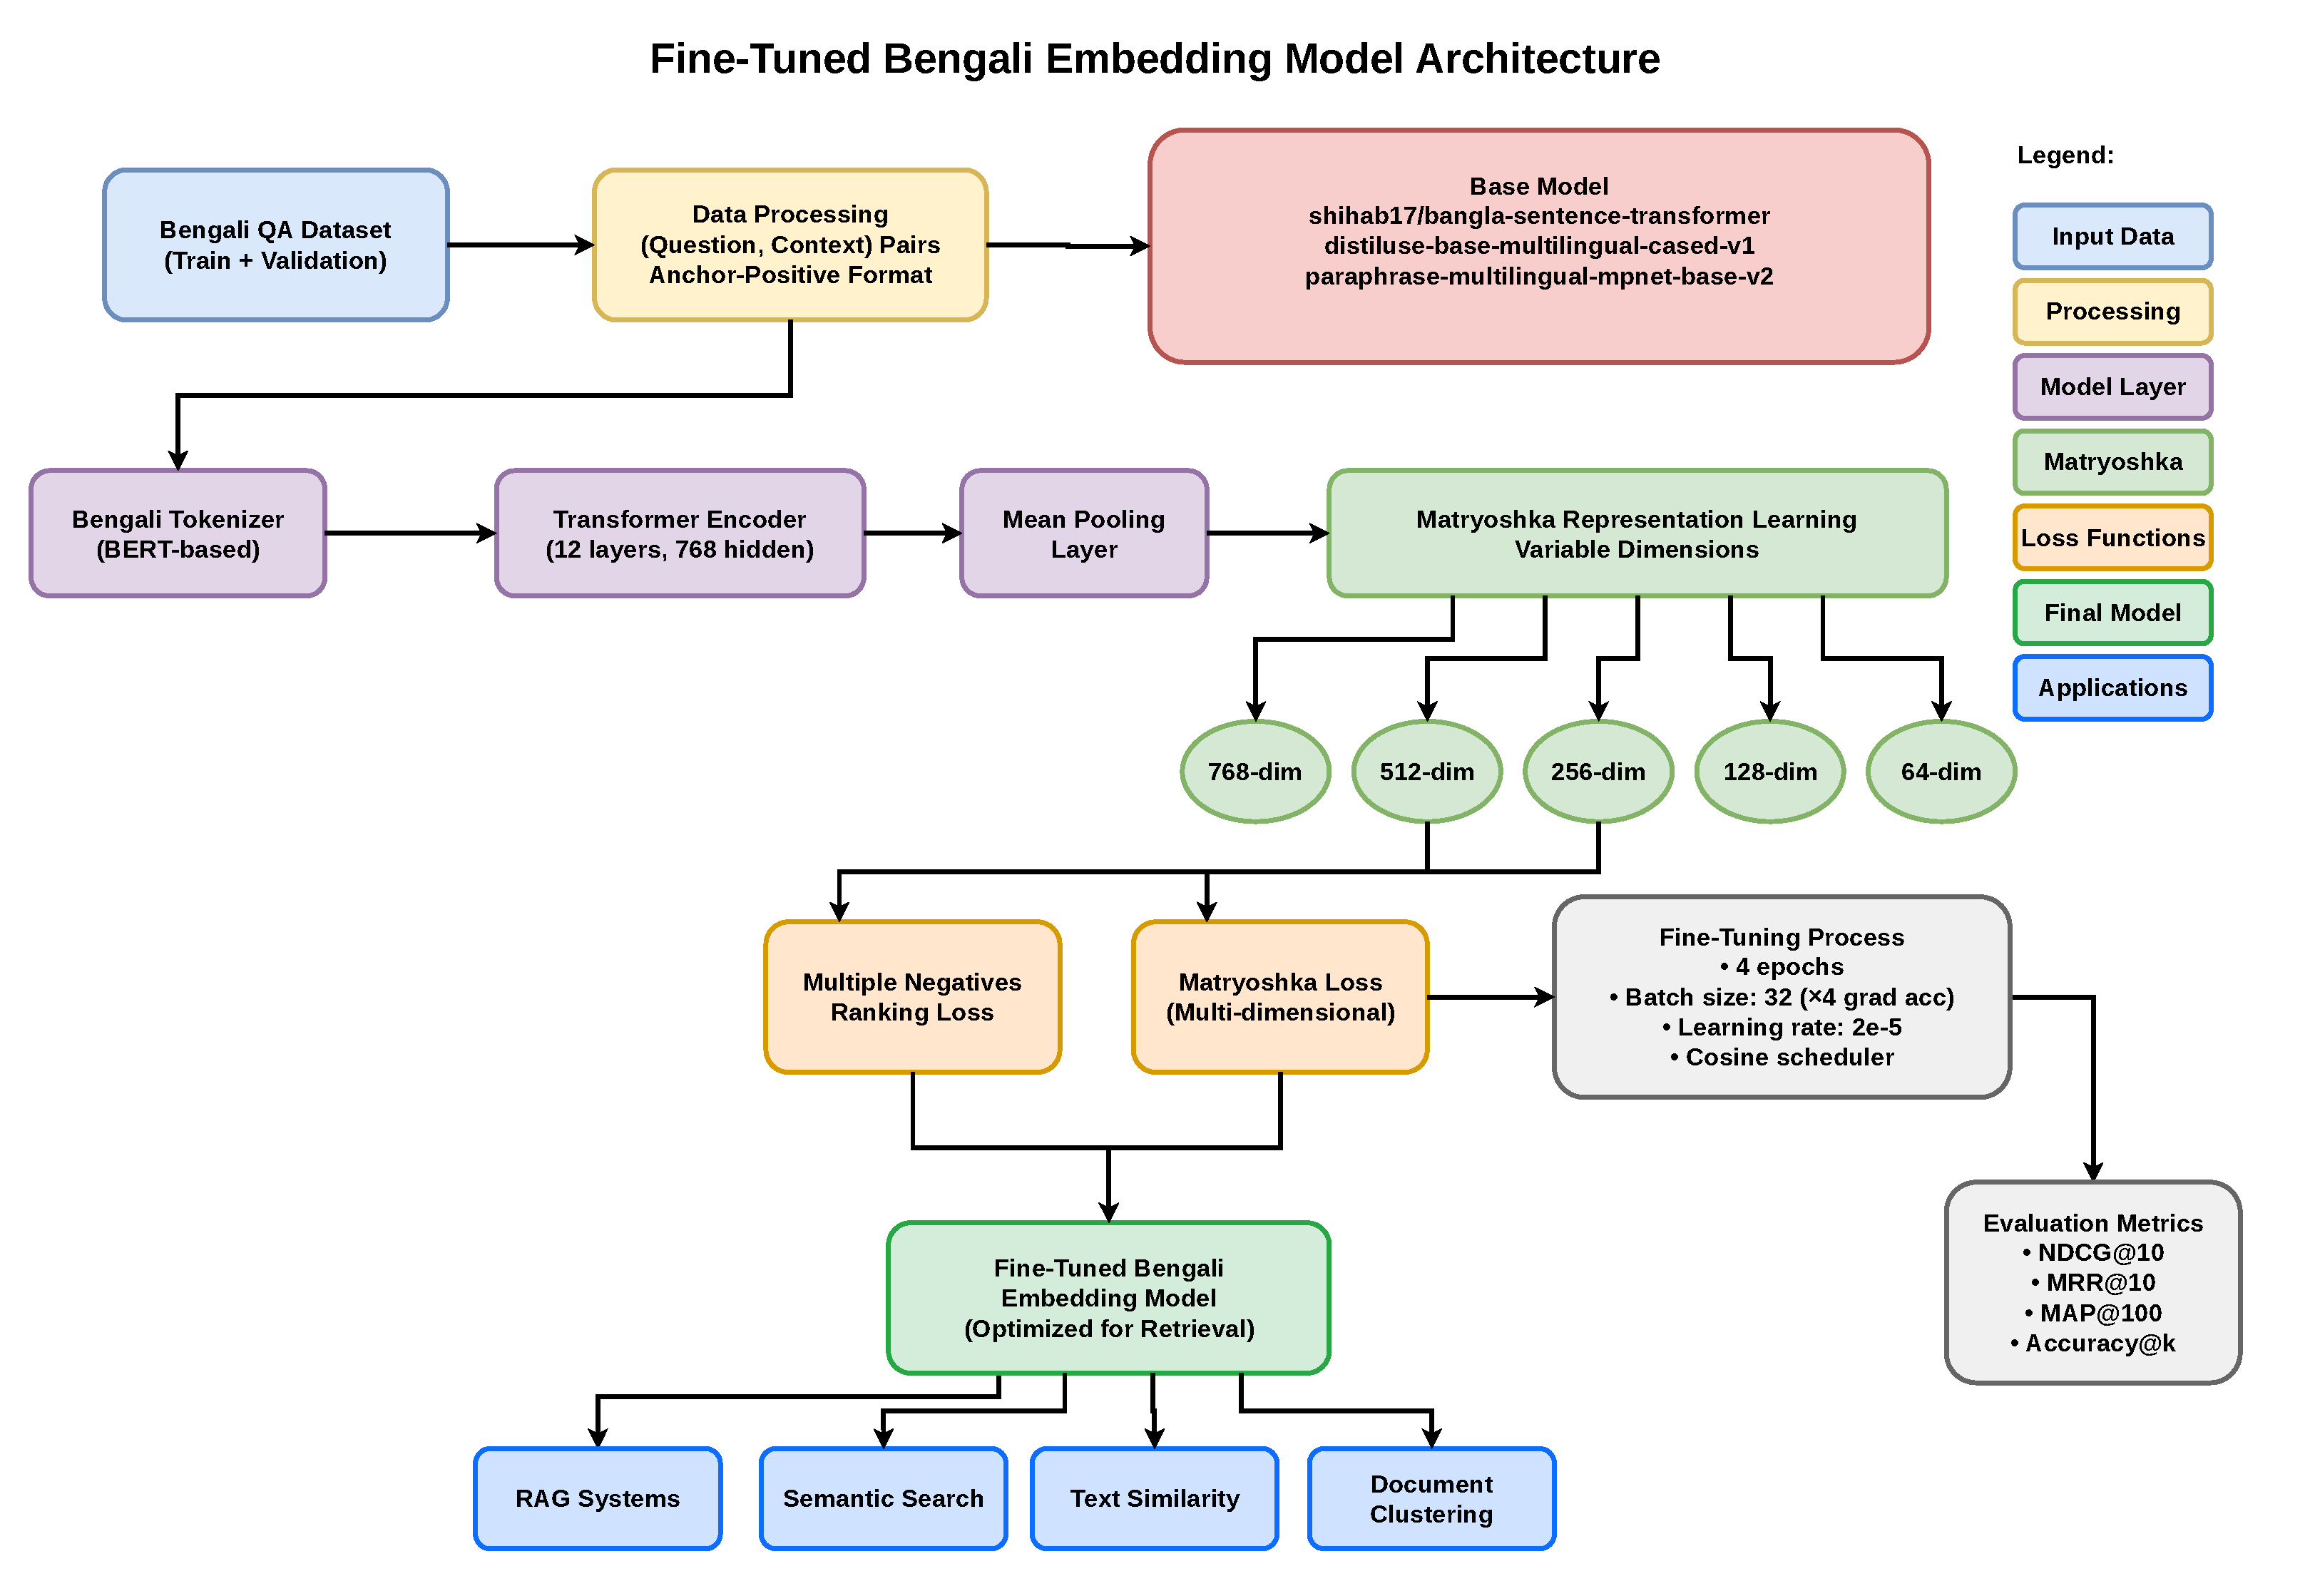
\includegraphics[width=\linewidth]{architechture.pdf}
    \caption{The comparative fine-tuning architecture. Three distinct base models are trained using a shared pipeline involving Siamese networks, Mean Pooling, and a Matryoshka-wrapped Multiple Negatives Ranking Loss function.}
    \label{fig:architecture}
    \Description{A block diagram showing the flow of data. Input sentences are fed into Base Models (Shihab17, Distiluse, MPNet). These pass through Siamese Networks with Shared Weights. The output goes to Mean Pooling, then to a Matryoshka Loss function layer which calculates Multiple Negatives Ranking Loss across varying dimensions.}
\end{figure}

\subsection{Base Models}
We selected three models representing different points on the efficiency-performance spectrum.

\textit{shihab17/bangla-sentence-transformer:} A monolingual model based on the XLM-R architecture, created via multilingual knowledge distillation \cite{uddin2024bangla}. It represents the specialized Bengali approach, producing 768-dimensional vectors.

\textit{distiluse-base-multilingual-cased-v1:} A knowledge-distilled version of the Universal Sentence Encoder \cite{reimers2019sentencebert}. It produces 512-dimensional vectors and is designed for high-throughput, low-latency applications.

\textit{paraphrase-multilingual-mpnet-base-v2:} A model based on the MPNet architecture, trained on a massive multilingual corpus of paraphrase pairs \cite{reimers2019sentencebert}. It is generally regarded as having stronger semantic modeling capabilities than standard BERT or RoBERTa models.

\subsection{Dataset Preparation}
We utilized the BanglaRQA dataset \cite{ekram2022banglarqa}, comprising human-annotated questions and answers from Bengali Wikipedia. We combined the training and validation splits to create a training corpus of 8,573 positive pairs. Crucially, we filtered for answerable questions to ensure high-quality positive signals. The test set consisted of 1,405 held-out pairs.

\begin{table*}[ht!]
    \centering
    \caption{BanglaRQA Dataset Samples}
    \label{tab:banglarqa_samples}
    \small % Slightly smaller font to fit width
    \setlength\tabcolsep{3pt} % Reduce padding between columns
    \renewcommand{\arraystretch}{1.2} % Better row spacing
    
    % Using tabularx to fit exactly to text width
    \begin{tabularx}{\textwidth}{
        >{\raggedright\arraybackslash\scriptsize}p{1.2cm}   % Passage ID
        >{\raggedright\arraybackslash\scriptsize}p{1.5cm}   % Title
        >{\scriptsize}X                                      % Context (Takes remaining space)
        >{\raggedright\arraybackslash\scriptsize}p{1.2cm}   % Q. ID
        >{\raggedright\arraybackslash\scriptsize}p{2.2cm}   % Question
        >{\centering\arraybackslash\scriptsize}p{0.6cm}     % Ans?
        >{\raggedright\arraybackslash\scriptsize}p{1.0cm}   % Type
        >{\raggedright\arraybackslash\tiny}p{3.0cm}         % Answers (JSON)
    }
        \toprule
        \textbf{Pass ID} & \textbf{Title} & \textbf{Context (Truncated)} & \textbf{Q. ID} & \textbf{Question} & \textbf{Ans?} & \textbf{Type} & \textbf{Answers} \\
        \midrule
        
        % --- Row 1 ---
        bn\_wiki\_ 0981 
        & \bn{ইন্টেল কর্পোরেশন} 
        & \bn{২০০০ সালের পর, প্রসেসরের চাহিদা হ্রাস পায়। প্রতিযোগিরা, বিশেষ করে এএমডি শেয়ার বাজারের বড় অংশ অধিগ্রহণ করে। শুরুতে কম ক্ষমতার এবং মধ্যম ক্ষমতার প্রসেসর এবং ধীরে ধীরে পুরো পণ্যের বাজার এবং মূল বাজারে ইন্টেলের অবস্থান আশঙ্কাজনকহারে কমে যায়। [...]} 
        & bn\_wiki\_ 0981\_01 
        & \bn{কত সালের পর, প্রসেসরের চাহিদা হ্রাস পায়?} 
        & 1 
        & factoid 
        & \ttfamily \{ "text": ["\bn{২০০০}", "\bn{২০০০}"], "type": ["single span", "single span"] \} \\
        \midrule
        
        % --- Row 2 ---
        bn\_wiki\_ 0656 
        & \bn{উবুন্টু (লিনাক্স)} 
        & \bn{উবুন্টু ইনস্টল করার জন্য সাধারণভাবে লাইভ সিডি ব্যবহার করা হয়। উবুন্টু অপারেটিং সিস্টেমটি ইনস্টল করা ছাড়াই সরাসরি সিডি থেকে ব্যবহার করা যায়। তবে লাইভ সিডি ব্যবহার করা হলে পূর্ণাঙ্গ অপারেটিং সিস্টেমের অনেক সুবিধাই এখানে পাওয়া যাবে না। [...]} 
        & bn\_wiki\_ 0656\_02 
        & \bn{কি নামে উবুন্টু ওএস ইনস্টল করতে সফটওয়্যার ব্যবহার করা হয়?} 
        & 0 
        & factoid 
        & \ttfamily \{ "text": ["", ""], "type": ["", ""] \} \\

        \bottomrule
    \end{tabularx}
\end{table*}

\subsection{Fine-tuning Strategy}
We employed a Siamese network structure with shared weights. The training objective was a summation of Multiple Negatives Ranking Loss (MNRL) calculated across varying dimensions, facilitated by Matryoshka Representation Learning.

MNRL treats the corresponding context for a question as the positive sample and all other contexts in the batch as negatives. The Matryoshka Loss wraps this objective, calculating the loss at dimensions $\{d_{max}, \dots, 64\}$. This forces the model to encode the most salient semantic information into the first 64 dimensions.

\section{Quantitative Evaluation}

We evaluated the models on the BanglaRQA test set using standard Information Retrieval metrics. Below we define the key metrics used in our analysis: Accuracy@k, Mean Reciprocal Rank (MRR), Mean Average Precision (MAP), and Normalized Discounted Cumulative Gain (NDCG). Let $Q$ be the set of all queries in the test set.

\begin{itemize}
    \item \textbf{Accuracy@k:} This metric measures the proportion of queries for which at least one correct document is found within the top $k$ retrieved results. It is a simple measure of success within a fixed retrieval window.
    
    \item \textbf{Mean Reciprocal Rank (MRR):} MRR evaluates how quickly the system finds the first relevant document. For each query, the reciprocal rank is the inverse of the rank of the first correct answer ($1/\text{rank}_i$). If no correct document is retrieved, the reciprocal rank is 0. The MRR is the average of these values across all queries.
    \begin{equation}
        \text{MRR} = \frac{1}{|Q|} \sum_{i=1}^{|Q|} \frac{1}{\text{rank}_i}
    \end{equation}
    
    \item \textbf{Mean Average Precision (MAP):} MAP provides a single-figure measure of quality across recall levels. For a single query $q$, Average Precision (AP) is the average of precision values calculated at each point a relevant document is found in the ranked list. MAP is the mean of these AP scores over all queries.
    \begin{equation}
        \text{AP}(q) = \frac{\sum_{k=1}^{n} (P(k) \times \text{rel}(k))}{\text{number of relevant documents for } q}
    \end{equation}
    \begin{equation}
        \text{MAP} = \frac{1}{|Q|} \sum_{q \in Q} \text{AP}(q)
    \end{equation}
    where $n$ is the number of retrieved documents, $P(k)$ is the precision at cutoff $k$, and $\text{rel}(k)$ is an indicator function that is 1 if the item at rank $k$ is relevant, and 0 otherwise.

    \item \textbf{Normalized Discounted Cumulative Gain (NDCG):} NDCG evaluates the quality of a ranking by considering the graded relevance of documents and penalizing relevant documents that appear lower in the list. It is calculated by dividing the Discounted Cumulative Gain (DCG) by the Ideal DCG (IDCG), which represents the gain of a perfect ranking. This normalization ensures the score is between 0 and 1.
    \begin{equation}
        \text{DCG}_k = \sum_{i=1}^{k} \frac{\text{rel}_i}{\log_2(i+1)}
    \end{equation}
    \begin{equation}
        \text{NDCG}_k = \frac{\text{DCG}_k}{\text{IDCG}_k}
    \end{equation}
    where $\text{rel}_i$ is the relevance score of the document at position $i$ (in our case, 1 for relevant, 0 for not).
\end{itemize}

\subsection{Performance Comparison}
The comprehensive results of our experiments are visualized in Figure \ref{fig:bar_comparison}. The \texttt{mpnet-base} model (green bars) emerged as the clear leader across all four metrics. Even at lower dimensions, it consistently outperformed the monolingual \texttt{shihab17} (blue) and distilled \texttt{distiluse} (red) models.

Table \ref{tab:comprehensive_comparison} details the specific improvements. The \texttt{distiluse} model, while efficient, started with a negligible baseline performance (NDCG@10 of 0.0037). Fine-tuning resurrected this model, bringing it to a respectable NDCG@10 of 0.4213. The monolingual \texttt{shihab17} model showed strong gains, improving to 0.5638. However, \texttt{mpnet} achieved the highest scores, with an NDCG@10 of 0.6139 and an Accuracy@1 of 54.36\%.

\begin{figure*}[ht!]
    \centering
    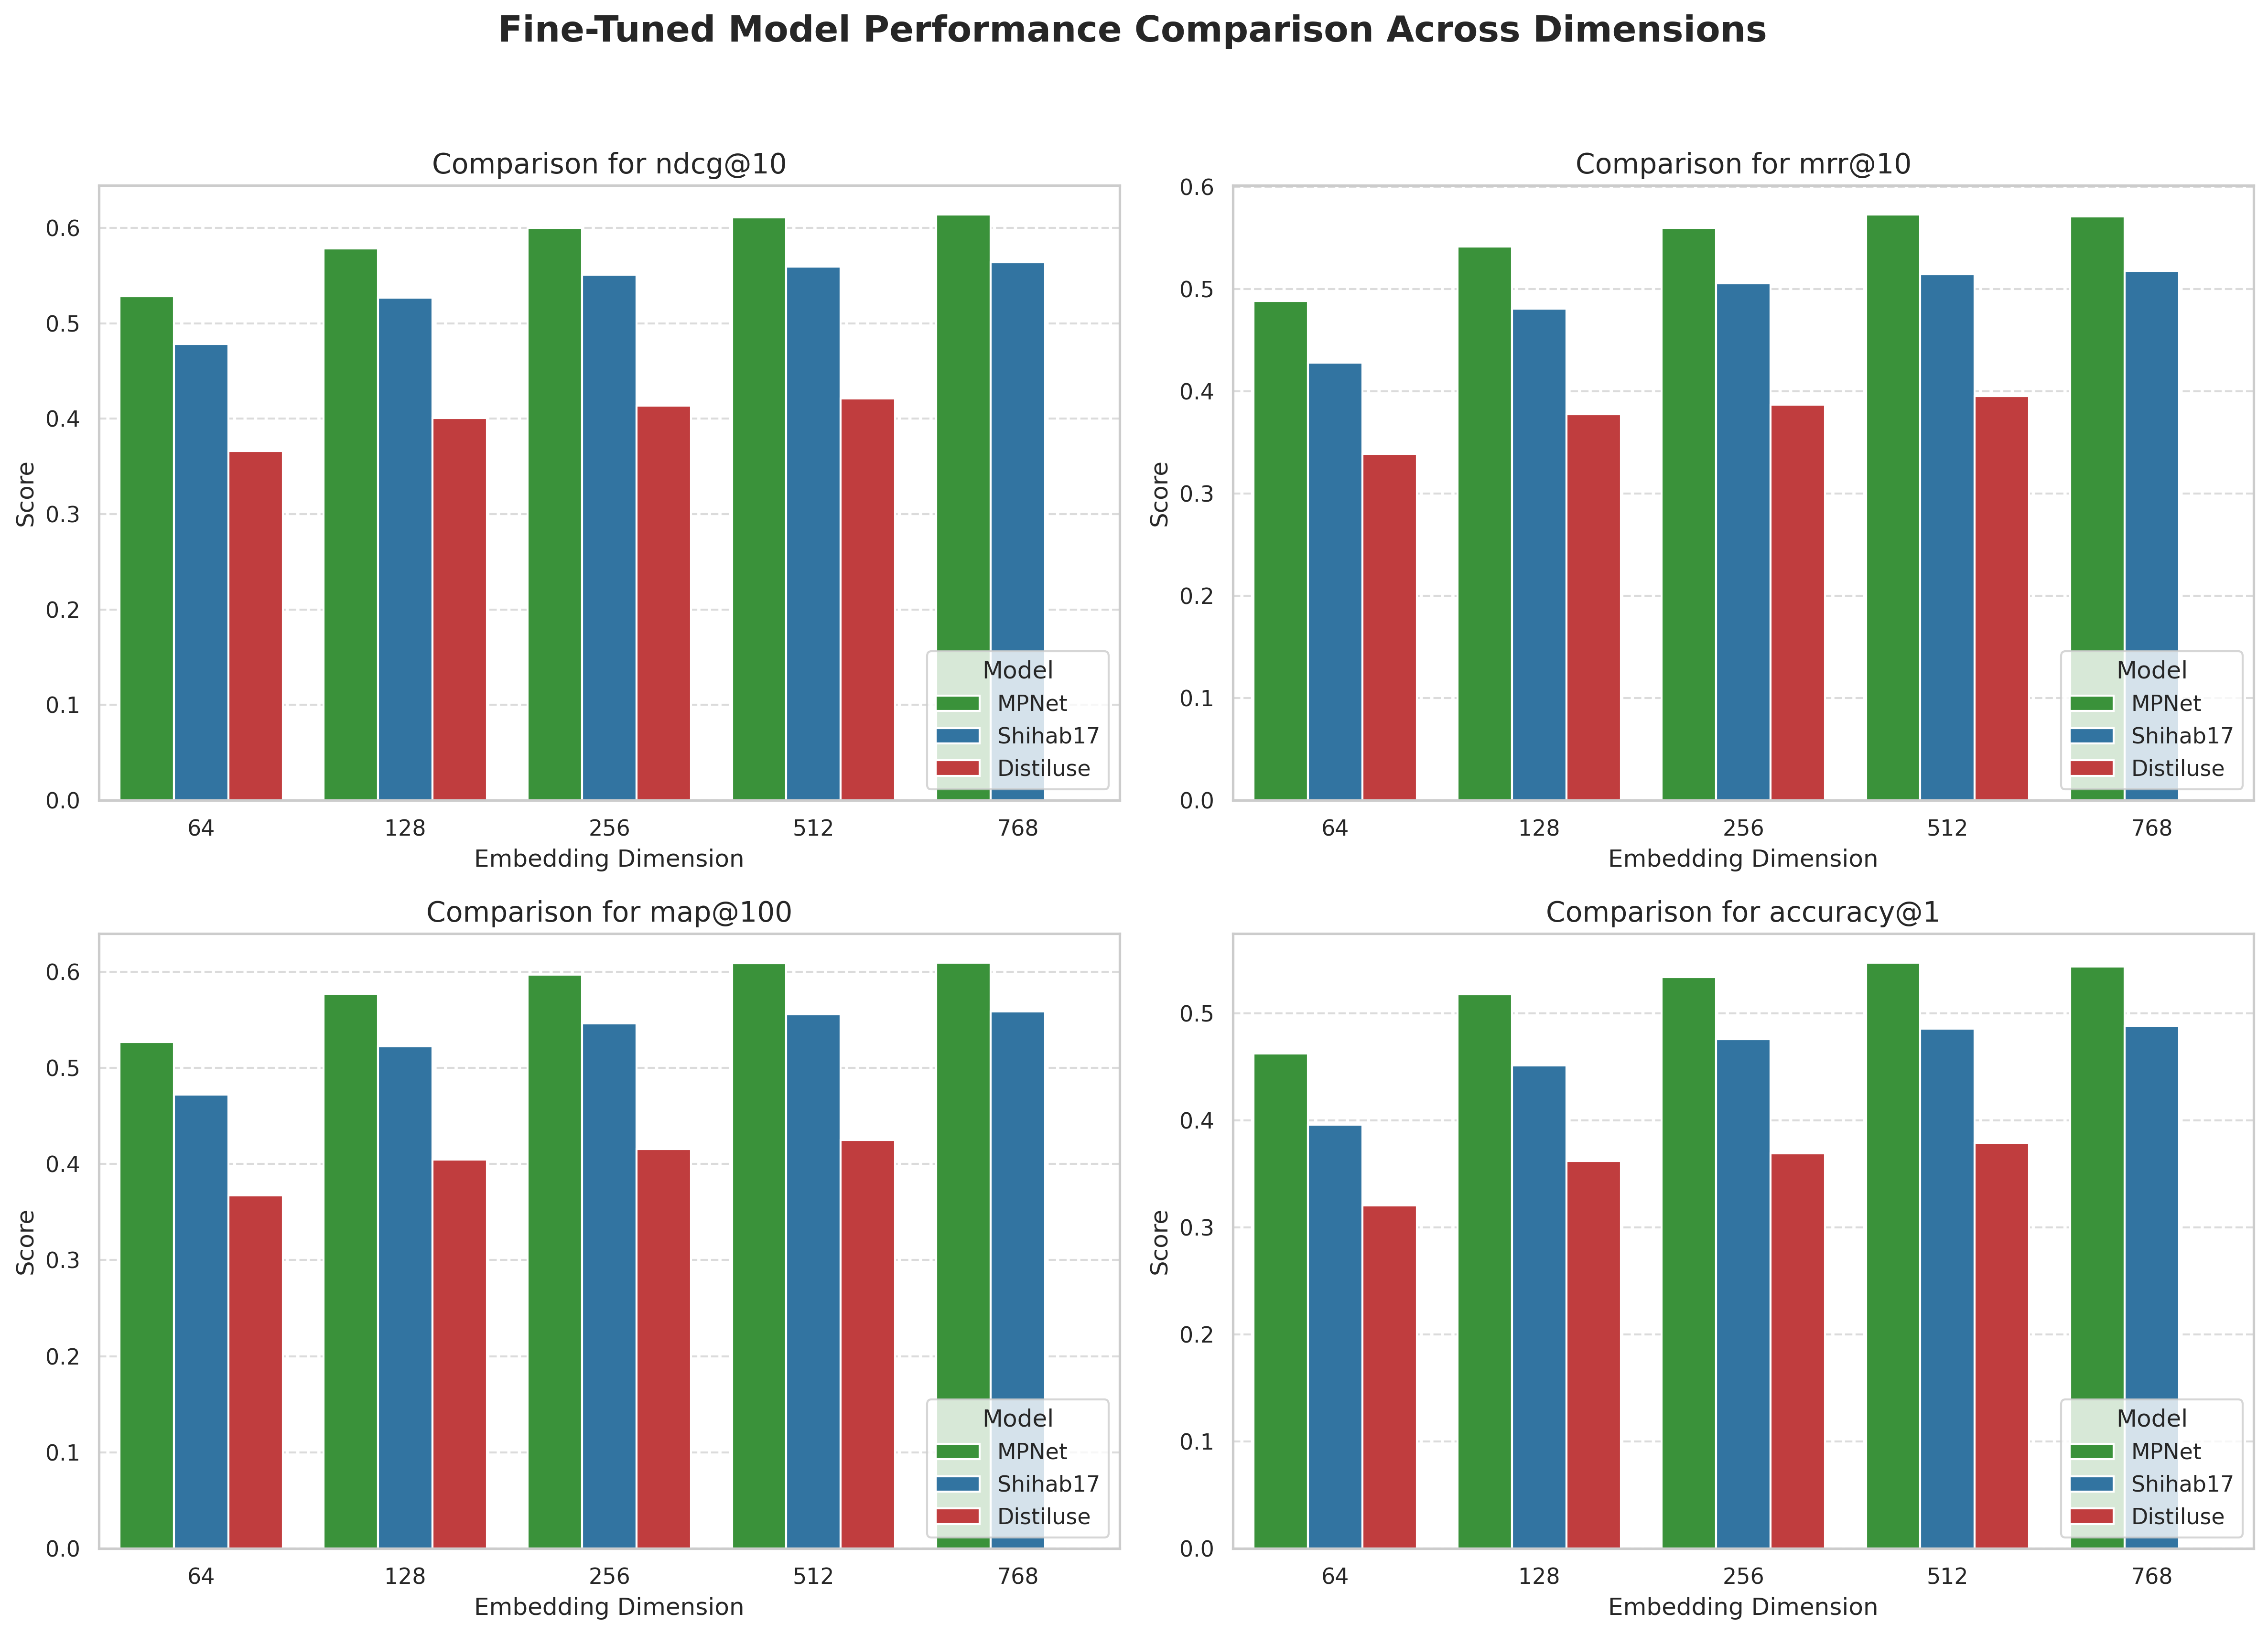
\includegraphics[width=0.95\textwidth]{model_comparison_results_high_dpi.png}
    \caption{Fine-Tuned Model Performance Comparison Across Dimensions. The MPNet model (green) demonstrates superior performance across NDCG@10, MRR@10, MAP@100, and Accuracy@1, maintaining its lead even as embedding dimensions are reduced.}
    \label{fig:bar_comparison}
    \Description{A bar chart comparing three models: shihab17, distiluse, and mpnet across four metrics. Green bars (mpnet) are consistently higher than blue (shihab17) and red (distiluse) bars.}
\end{figure*}



\begin{figure*}[htbp]
    \centering
    % Adjust width=1.0\textwidth if you want it to span two columns, 
    % or width=1.0\linewidth for a single column.
    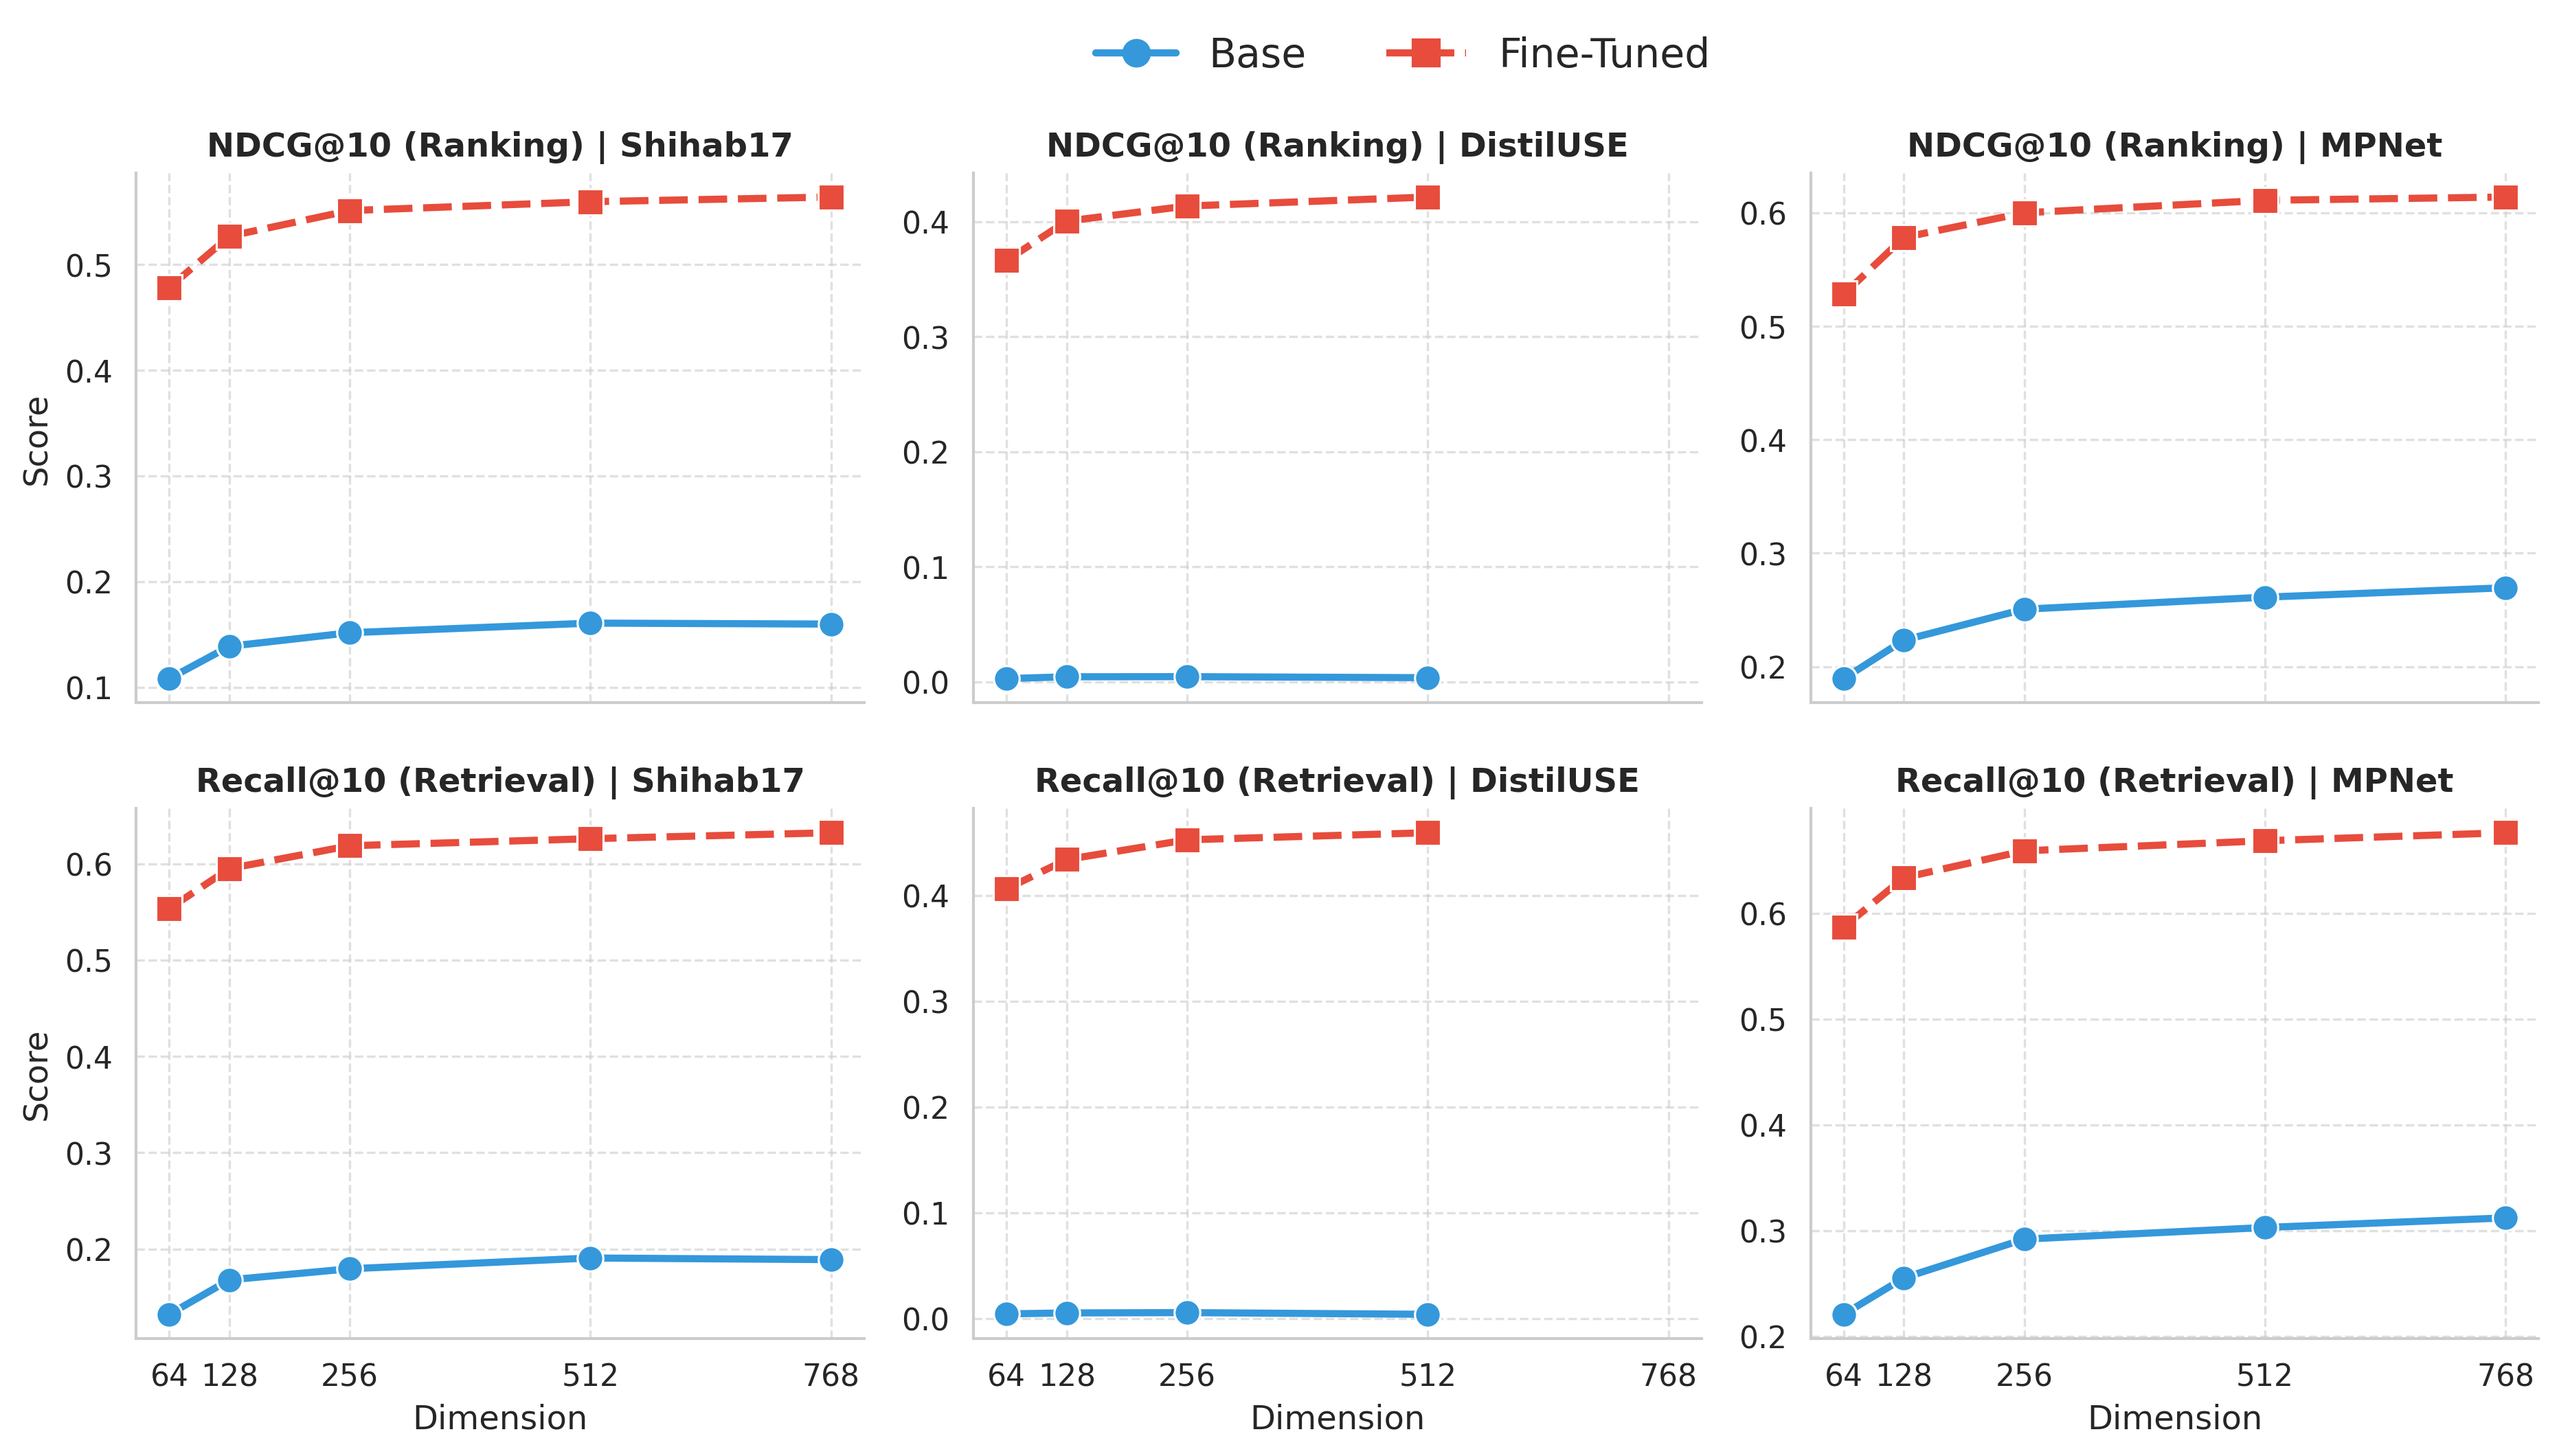
\includegraphics[width=1.0\textwidth]{model_comparison_facet_grid.png}
    \caption{\textbf{Impact of fine-tuning on semantic search performance across varying dimensions (64d--768d).} 
    The comparison highlights the efficacy gap between Base (Blue/Circle) and Fine-Tuned (Red/Square) models. 
    The top row displays Ranking Quality (\textbf{NDCG@10}), while the bottom row displays Retrieval Coverage (\textbf{Recall@10}). 
    Fine-tuned models demonstrate superior performance and robustness to dimensionality reduction compared to pre-trained base models.}
    \label{fig:model_comparison}
\end{figure*}


To rigorously evaluate the efficacy of our fine-tuning approach, we conducted a comparative analysis against the pre-trained base models across varying vector dimensions ranging from $64d$ to $768d$. As illustrated in Fig.~\ref{fig:model_comparison}, the fine-tuned models (indicated by the red squares) consistently outperform their base counterparts (blue circles) by a significant margin across all three architectures.

In terms of ranking quality (NDCG@10), the MPNet and Shihab17 (BanglaBERT) models show substantial gains. For instance, the fine-tuned MPNet achieves an NDCG@10 score of $0.6139$ at 768 dimensions, compared to $0.2695$ for the base model—an improvement of approximately $127\%$. 

Most notably, the DistilUSE base model exhibited near-zero performance ($<0.01$ across all metrics), indicating a lack of semantic alignment for the target language in its pre-trained state. However, post-fine-tuning, the model recovered to a competitive NDCG@10 of $0.4213$, demonstrating that our training methodology successfully aligned the multilingual vector space.

Furthermore, Fig.~\ref{fig:model_comparison} demonstrates the robustness of the fine-tuned models to dimensionality reduction. While performance naturally degrades as dimensions are reduced towards $64d$, the fine-tuned models maintain high utility. Specifically, the fine-tuned Shihab17 model at $64d$ retains an NDCG score of $0.4783$, which surpasses the performance of the full $768d$ base MPNet model. This suggests that our fine-tuned models are highly effective for resource-constrained environments where low-dimensional embeddings are required for storage efficiency.


\begin{table*}[!htbp]
    \centering
    \caption{Comparative Performance of Fine-Tuned (FT) Models vs. Baselines at Maximum Dimensions. The best scores are highlighted in \textbf{bold}. The $\dagger$ symbol indicates that the best model (MPNet) is statistically significantly better than the second-best model (Shihab17) with $p < 0.001$.}
    \label{tab:comprehensive_comparison}
    \resizebox{\textwidth}{!}{%
    \begin{tabular}{llcccccccccccc}
        \toprule
        \multirow{2}{*}{\textbf{Model}} & \multirow{2}{*}{\textbf{Dim}} & \multicolumn{2}{c}{\textbf{NDCG@10}} & \multicolumn{2}{c}{\textbf{MRR@10}} & \multicolumn{2}{c}{\textbf{MAP@100}} & \multicolumn{2}{c}{\textbf{Accuracy@10}} & \multicolumn{2}{c}{\textbf{Precision@10}} & \multicolumn{2}{c}{\textbf{Recall@10}} \\
        \cmidrule(lr){3-4} \cmidrule(lr){5-6} \cmidrule(lr){7-8} \cmidrule(lr){9-10} \cmidrule(lr){11-12} \cmidrule(lr){13-14}
         & & Base & FT & Base & FT & Base & FT & Base & FT & Base & FT & Base & FT \\
        \midrule
        DistilUSE & 512d & 0.0037 & 0.4213 & 0.0036 & 0.3955 & 0.0056 & 0.4248 & 0.0044 & 0.4698 & 0.0014 & 0.1770 & 0.0040 & 0.4592 \\
        Shihab17 & 768d & 0.1599 & 0.5638 & 0.1411 & 0.5179 & 0.1651 & 0.5586 & 0.1993 & 0.6557 & 0.0715 & 0.2424 & 0.1889 & 0.6323 \\
        MPNet & 768d & 0.2695 & \textbf{0.6139}$^\dagger$ & 0.2413 & \textbf{0.5712}$^\dagger$ & 0.2761 & \textbf{0.6094}$^\dagger$ & 0.3283 & \textbf{0.6913}$^\dagger$ & 0.1201 & \textbf{0.2593}$^\dagger$ & 0.3120 & \textbf{0.6762}$^\dagger$ \\
        \bottomrule
    \end{tabular}%
    }
\end{table*}


Table \ref{tab:comprehensive_comparison} presents a detailed breakdown of the results at the maximum embedding dimensions available for each architecture. Across all metrics, fine-tuning delivered clear performance gains.

Most strikingly, the DistilUSE model moved from an almost unusable baseline (NDCG of 0.0037) to a strong post–fine-tuning score of 0.4213. MPNet reached the best overall performance, with an Accuracy@10 of 0.6913—meaning the correct item appeared in the top ten nearly 70\% of the time, up from 32\% in the base version. The Shihab17 model also saw a three-fold jump in Recall@10, rising from 0.1889 to 0.6323.




\subsection{Statistical Significance Analysis}

To ascertain that the performance superiority of the \texttt{mpnet} architecture is not merely an artifact of specific query variations or random initialization, we conducted a statistical significance test on the test set predictions. Given that information retrieval metrics such as NDCG are typically non-normally distributed, we employed the \textbf{Wilcoxon Signed-Rank Test}, a non-parametric paired difference test.

We formulated the null hypothesis ($H_0$) that there is no significant difference in the median retrieval performance between the best-performing model (\texttt{mpnet-ft}) and the runner-up models. We compared the per-query NDCG@10 scores across the $1,405$ test queries.

The results, summarized in Table~\ref{tab:significance}, strongly reject the null hypothesis. The fine-tuned \texttt{mpnet} model demonstrates a statistically significant improvement over the monolingual \texttt{shihab17} model ($p < 0.001$) and the distilled \texttt{distiluse} model ($p < 0.001$). The extremely low p-values (e.g., $1.0 \times 10^{-47}$ against DistilUSE) confirm that \texttt{mpnet}'s architectural advantages translate into robust, consistent gains across the vast majority of the test distribution.

\begin{table}[h]
    \centering
    \caption{Wilcoxon Signed-Rank Test Results (NDCG@10)}
    \label{tab:significance}
    \begin{tabular}{llcc}
        \toprule
        \textbf{Model A} & \textbf{Model B} & \textbf{Statistic} & \textbf{p-value} \\
        \midrule
        MPNet-FT & Shihab17-FT & $8.02 \times 10^3$ & $7.81 \times 10^{-6}$ \\
        MPNet-FT & DistilUSE-FT & $8.30 \times 10^3$ & $1.00 \times 10^{-47}$ \\
        Shihab17-FT & DistilUSE-FT & $1.12 \times 10^4$ & $5.35 \times 10^{-38}$ \\
        \bottomrule
    \end{tabular}
\end{table}


\subsection{Matryoshka Efficiency and Saturation}
A critical analysis of the results at lower dimensions highlights the success of the Matryoshka training strategy. As illustrated in the saturation curves in Figure \ref{fig:saturation}, all models exhibit a logarithmic growth in performance as dimensions increase, eventually reaching a plateau. The \texttt{mpnet} model (green line) consistently dominates across all dimensions. Notably, the "elbow" of the curve appears early; moving from 256 to 768 dimensions yields diminishing returns. Figure \ref{fig:dim_effect} further illustrates this saturation effect from a classification metric perspective, showing that individual scores for accuracy, f1, precision, and recall follow a similar logarithmic growth pattern, with most gains realized by the 512-dimension mark.

\begin{figure*}[ht!]
    \centering
    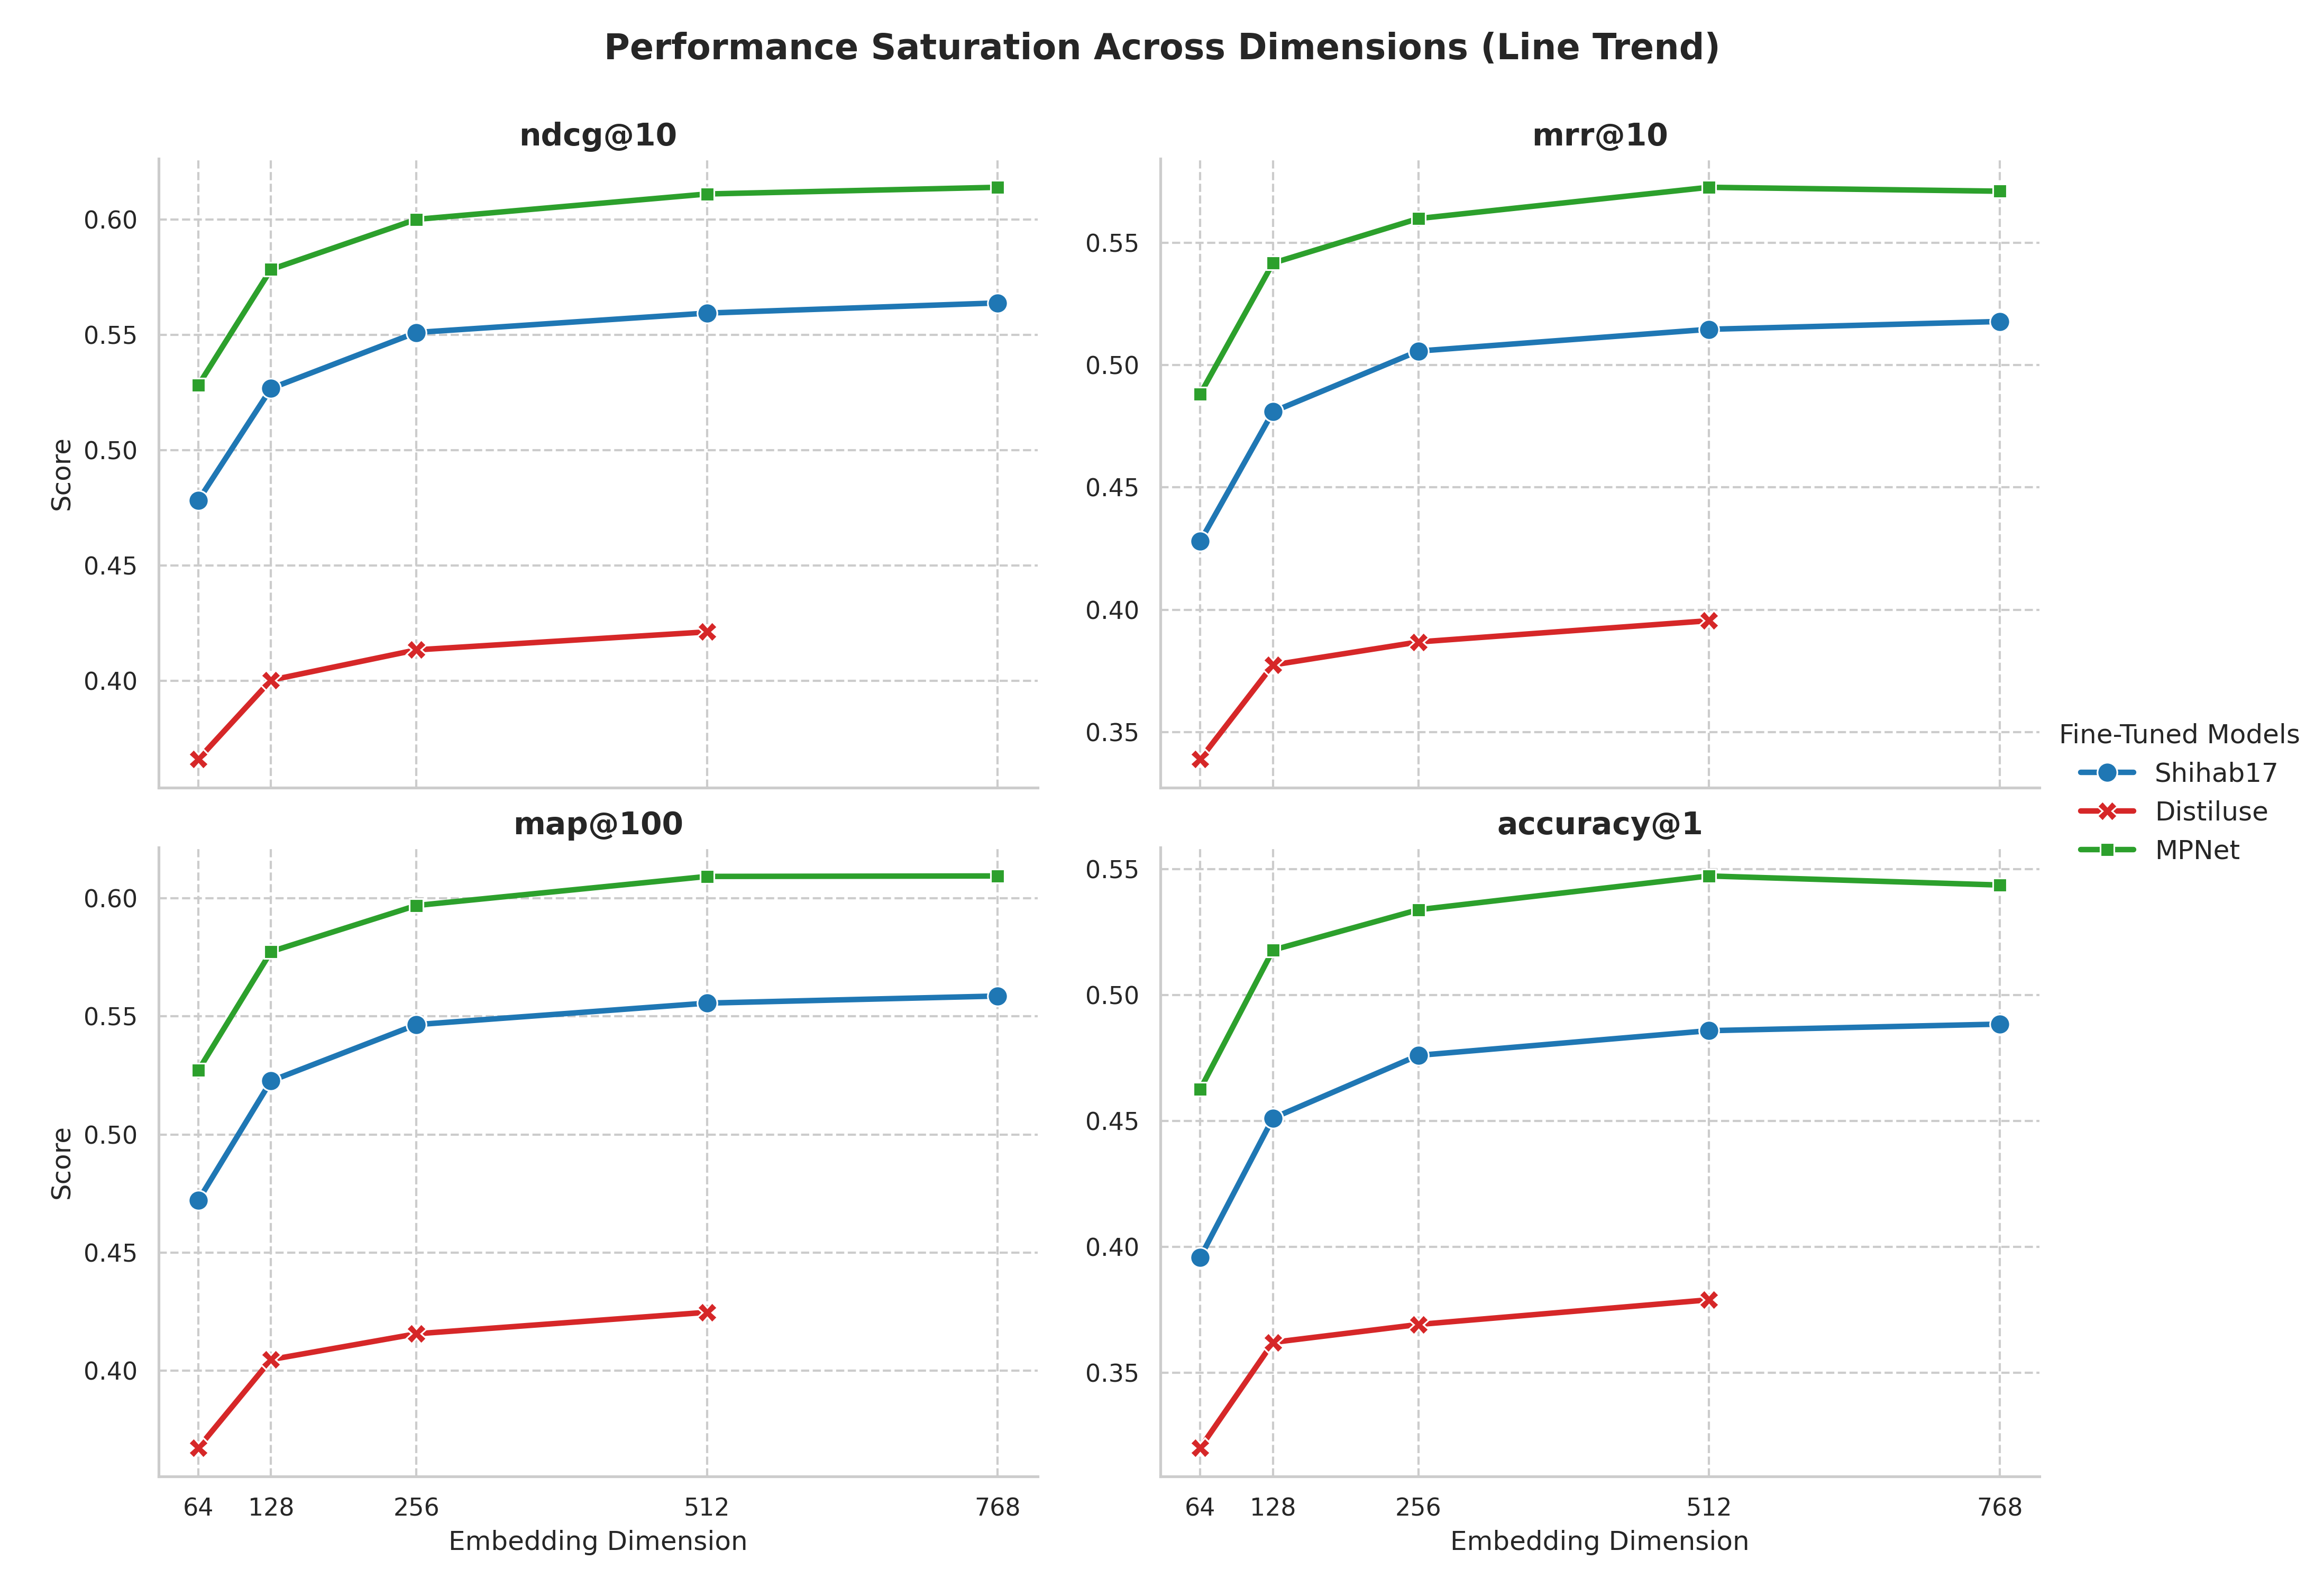
\includegraphics[width=0.9\textwidth]{paper_plot_saturation_lines.png}
    \caption{Performance saturation across dimensions for different metrics. The MPNet model demonstrates superior scaling, reaching near-peak performance earlier than the monolingual or distilled baselines.}
    \label{fig:saturation}
    \Description{Line graphs showing performance metrics vs. embedding dimensions. The X-axis represents dimensions (64 to 768), and the Y-axis represents the score. The green line for MPNet is above the others and flattens out after 256 dimensions.}
\end{figure*}

\begin{figure}[ht!]
    \centering
    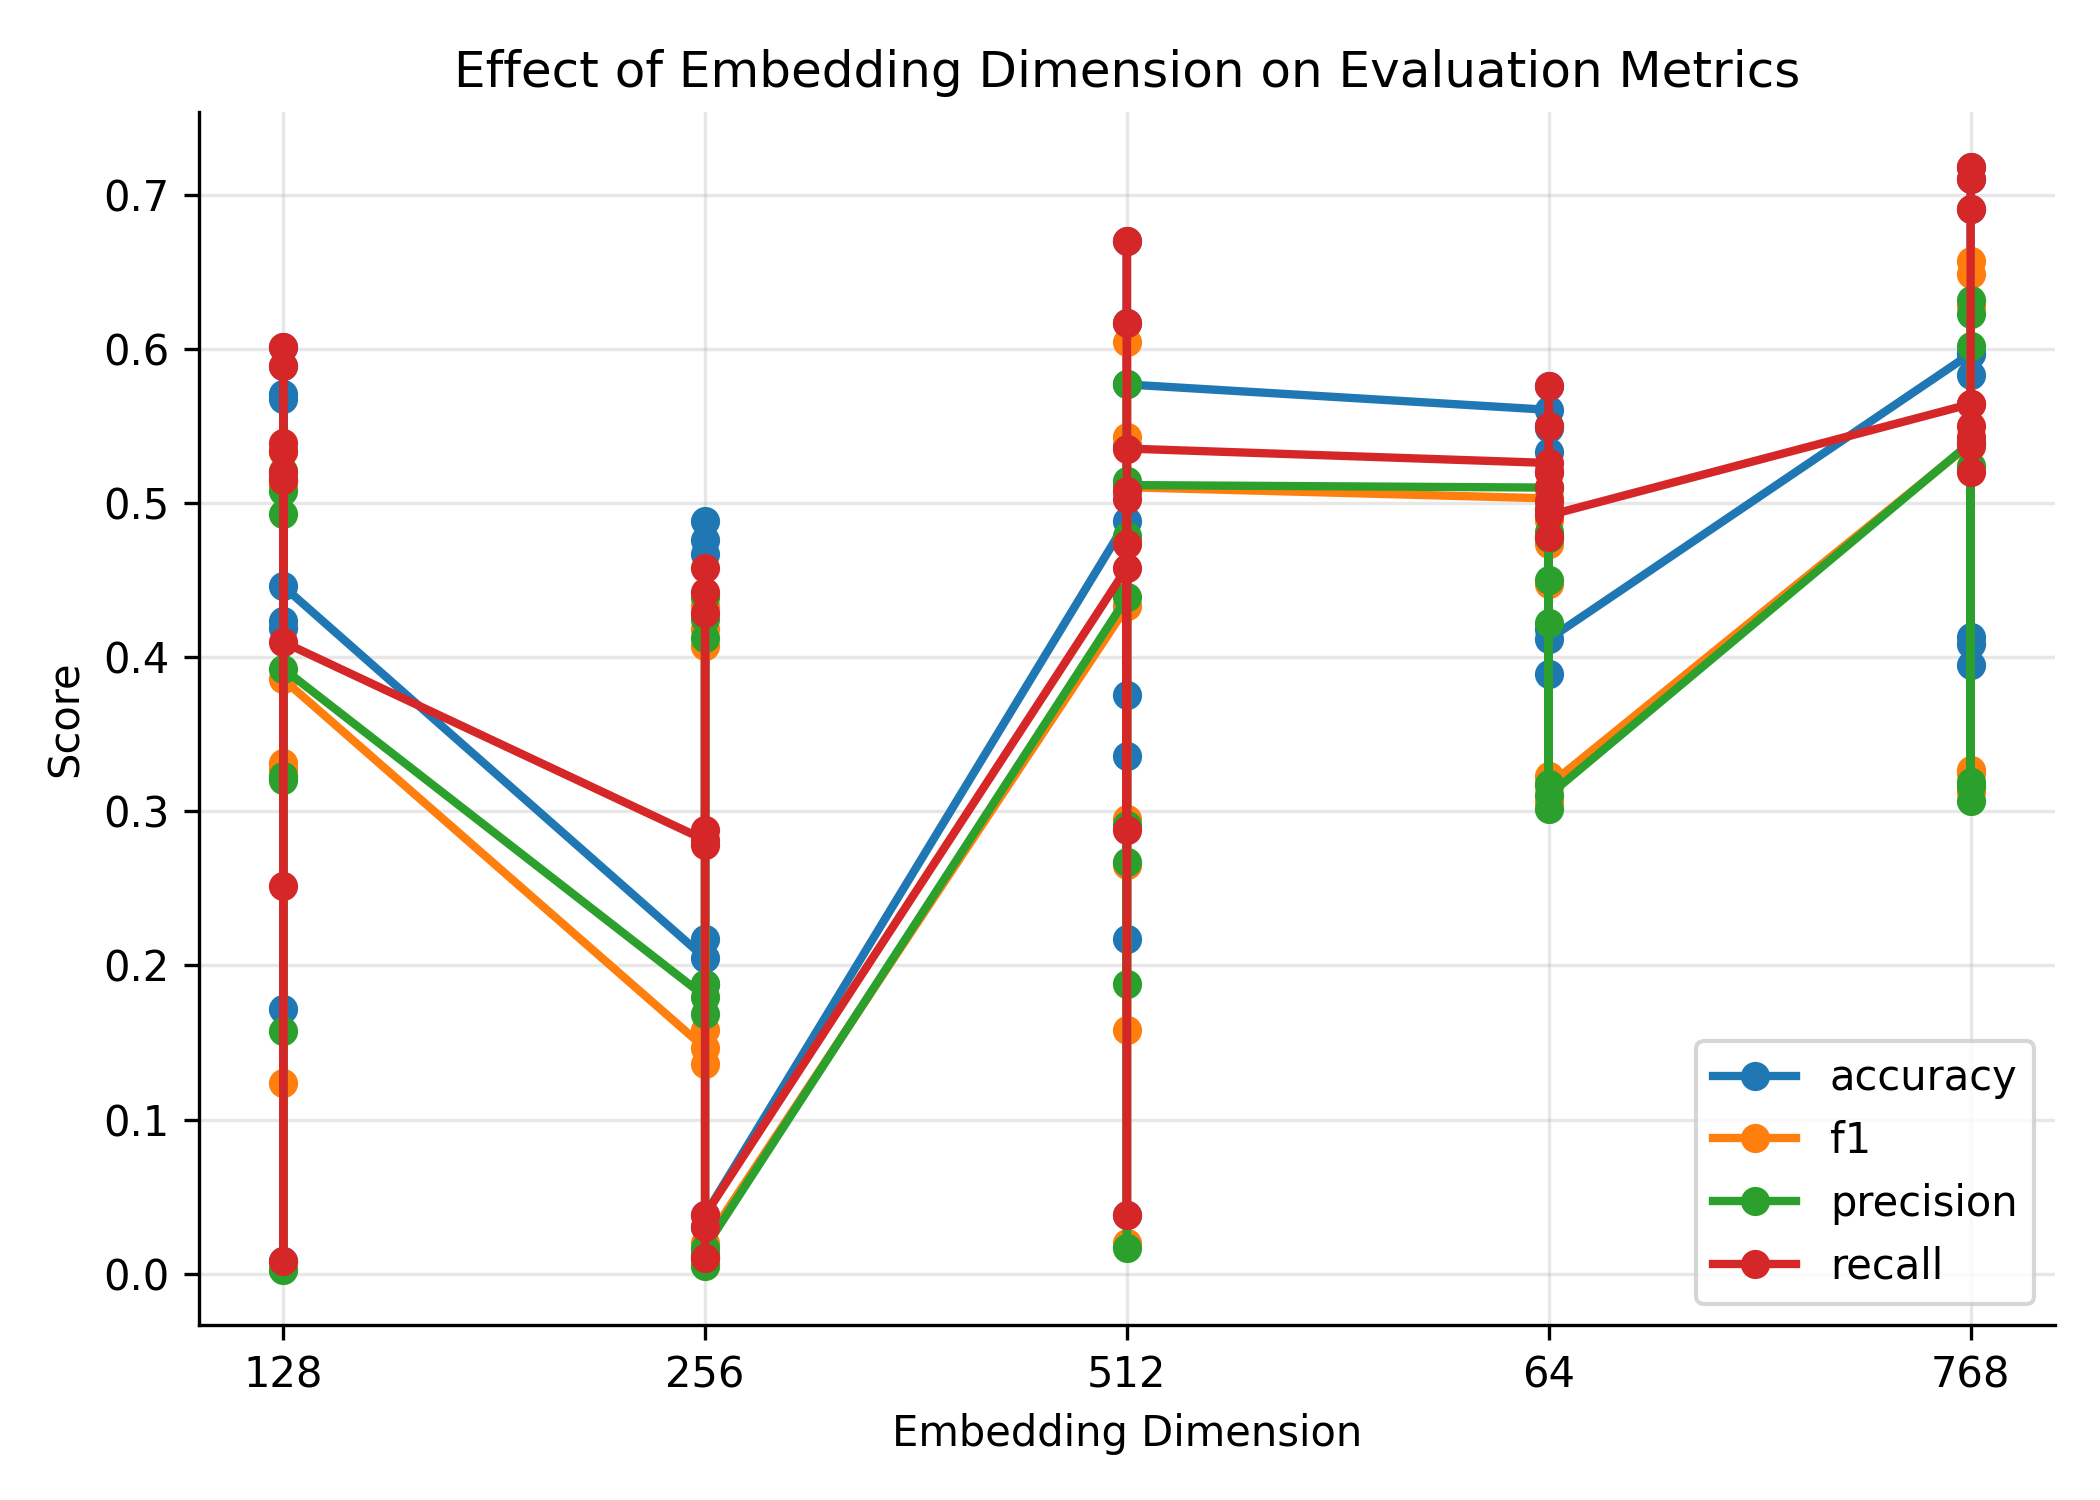
\includegraphics[width=0.8\linewidth]{embed_dim_vs_metrics.png}
    \caption{Effect of Embedding Dimension on Evaluation Metrics for the fine-tuned MPNet model. Performance across key metrics begins to plateau after 256-512 dimensions, reinforcing the effectiveness of Matryoshka Representation Learning.}
    \label{fig:dim_effect}
    \Description{A line chart with Embedding Dimension on the x-axis (from 128 to 768) and Score on the y-axis. Four colored lines with markers represent accuracy, f1, precision, and recall. All lines show a steep rise from 128 to 512 dimensions, after which they flatten, indicating diminishing returns for higher dimensions.}
\end{figure}

To quantify this efficiency, we analyzed the performance retention relative to the best-performing MPNet configuration (Figure \ref{fig:retention}). The results are striking: MPNet achieves over 95\% of its maximum capacity at just 128 dimensions. This implies that for large-scale Bengali retrieval systems, one can achieve state-of-the-art accuracy with a fraction of the storage usually necessary.

\begin{figure}[ht!]
    \centering
    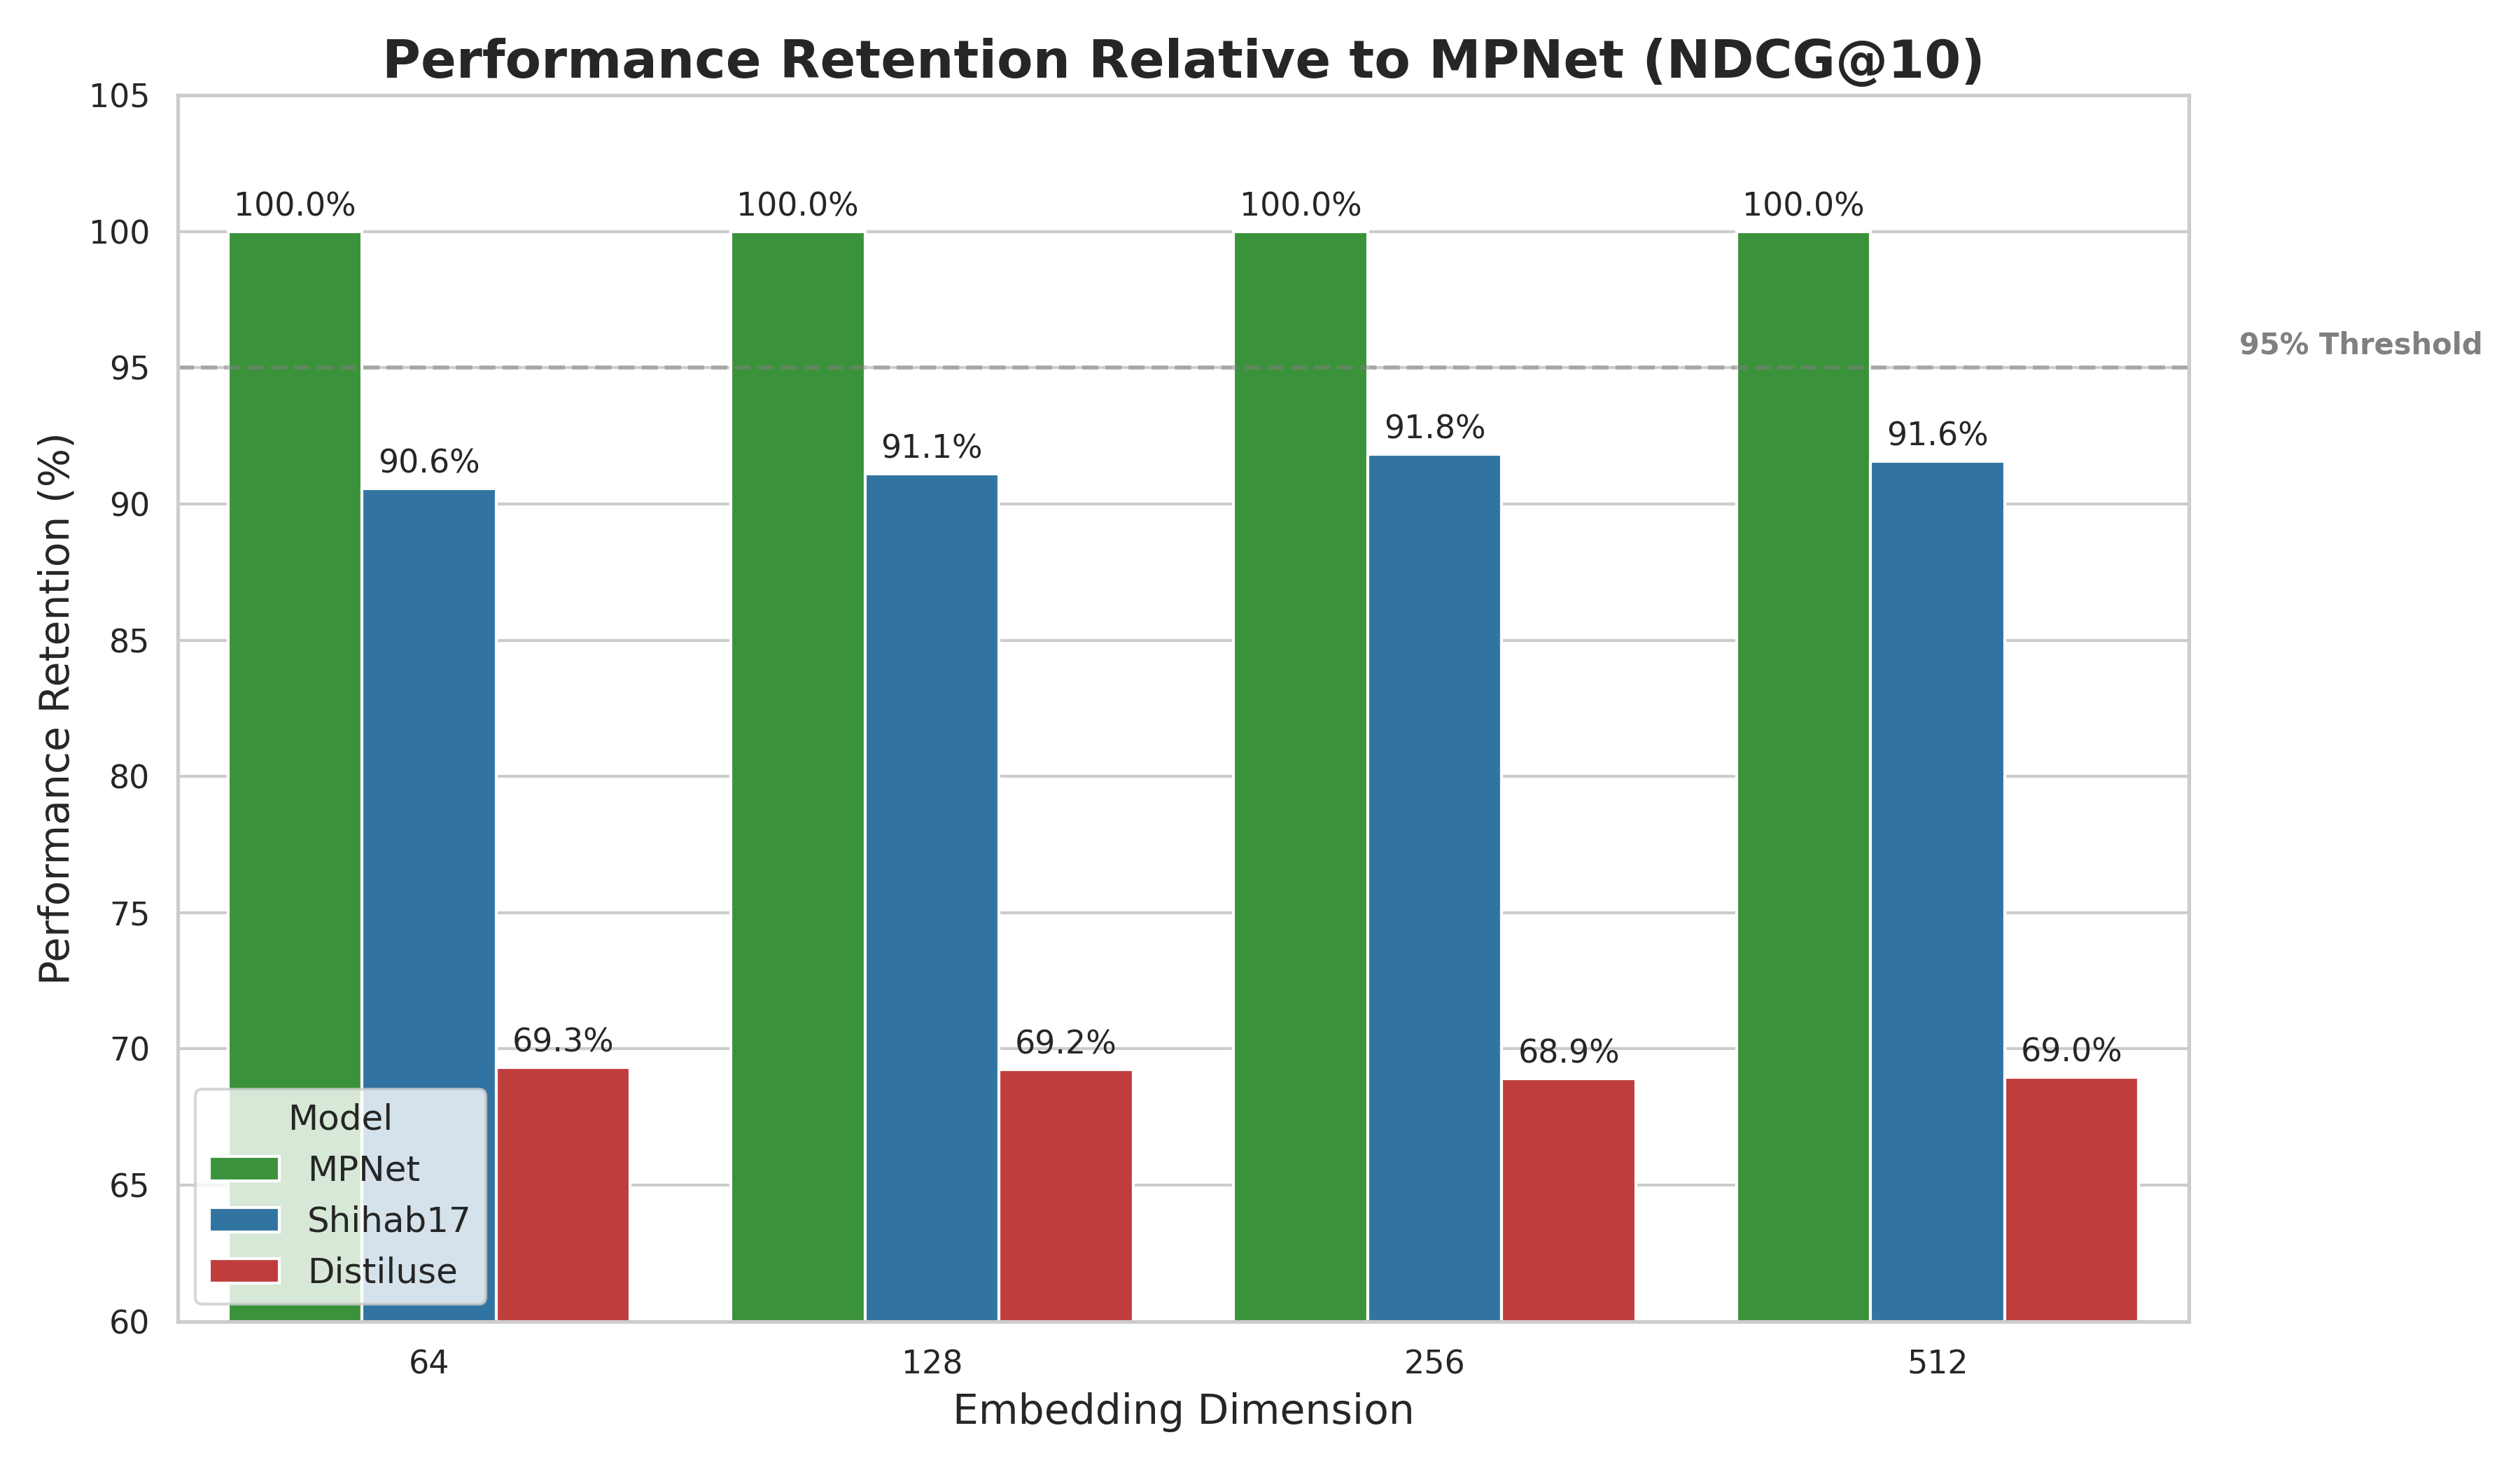
\includegraphics[width=\linewidth]{paper_plot_retention.png}
    \caption{Performance Retention Analysis (NDCG@10). Bars indicate the percentage of performance retained relative to the full-precision MPNet model. The dashed line indicates the 95\% efficiency threshold.}
    \label{fig:retention}
    \Description{A bar chart showing retention percentages. A horizontal dashed line marks the 95\% threshold. MPNet bars cross this threshold at low dimensions.}
\end{figure}

\subsection{Generalization on MTEB Benchmarks}
To assess the generalization capabilities of our fine-tuned models beyond the primary question-answering task, we evaluated them on a selection of Bengali tasks from the Massive Text Embedding Benchmark (MTEB). The selected tasks included `BengaliDocumentClassification.v2` (BDC), `BengaliHateSpeechClassification.v2` (BHSC), and the `Tatoeba` bitext retrieval task. This evaluation measures how well the semantic space learned on BanglaRQA transfers to broader classification and retrieval contexts.

The results, depicted in Figure \ref{fig:mteb_breakdown}, reinforce the superiority of the fine-tuned MPNet architecture. The model-wise breakdown clearly shows that MPNet consistently achieves the highest scores across all three datasets and nearly all evaluation metrics. While the monolingual `shihab17` model shows competitive performance, particularly on the classification tasks (BDC, BHSC), it does not reach the overall proficiency of MPNet. The `distiluse` model lags significantly behind both. This broader evaluation confirms that the architectural advantages of MPNet, enhanced by our fine-tuning strategy, translate into robust, general-purpose semantic representations for the Bengali language.

\begin{figure*}[ht!]
    \centering
    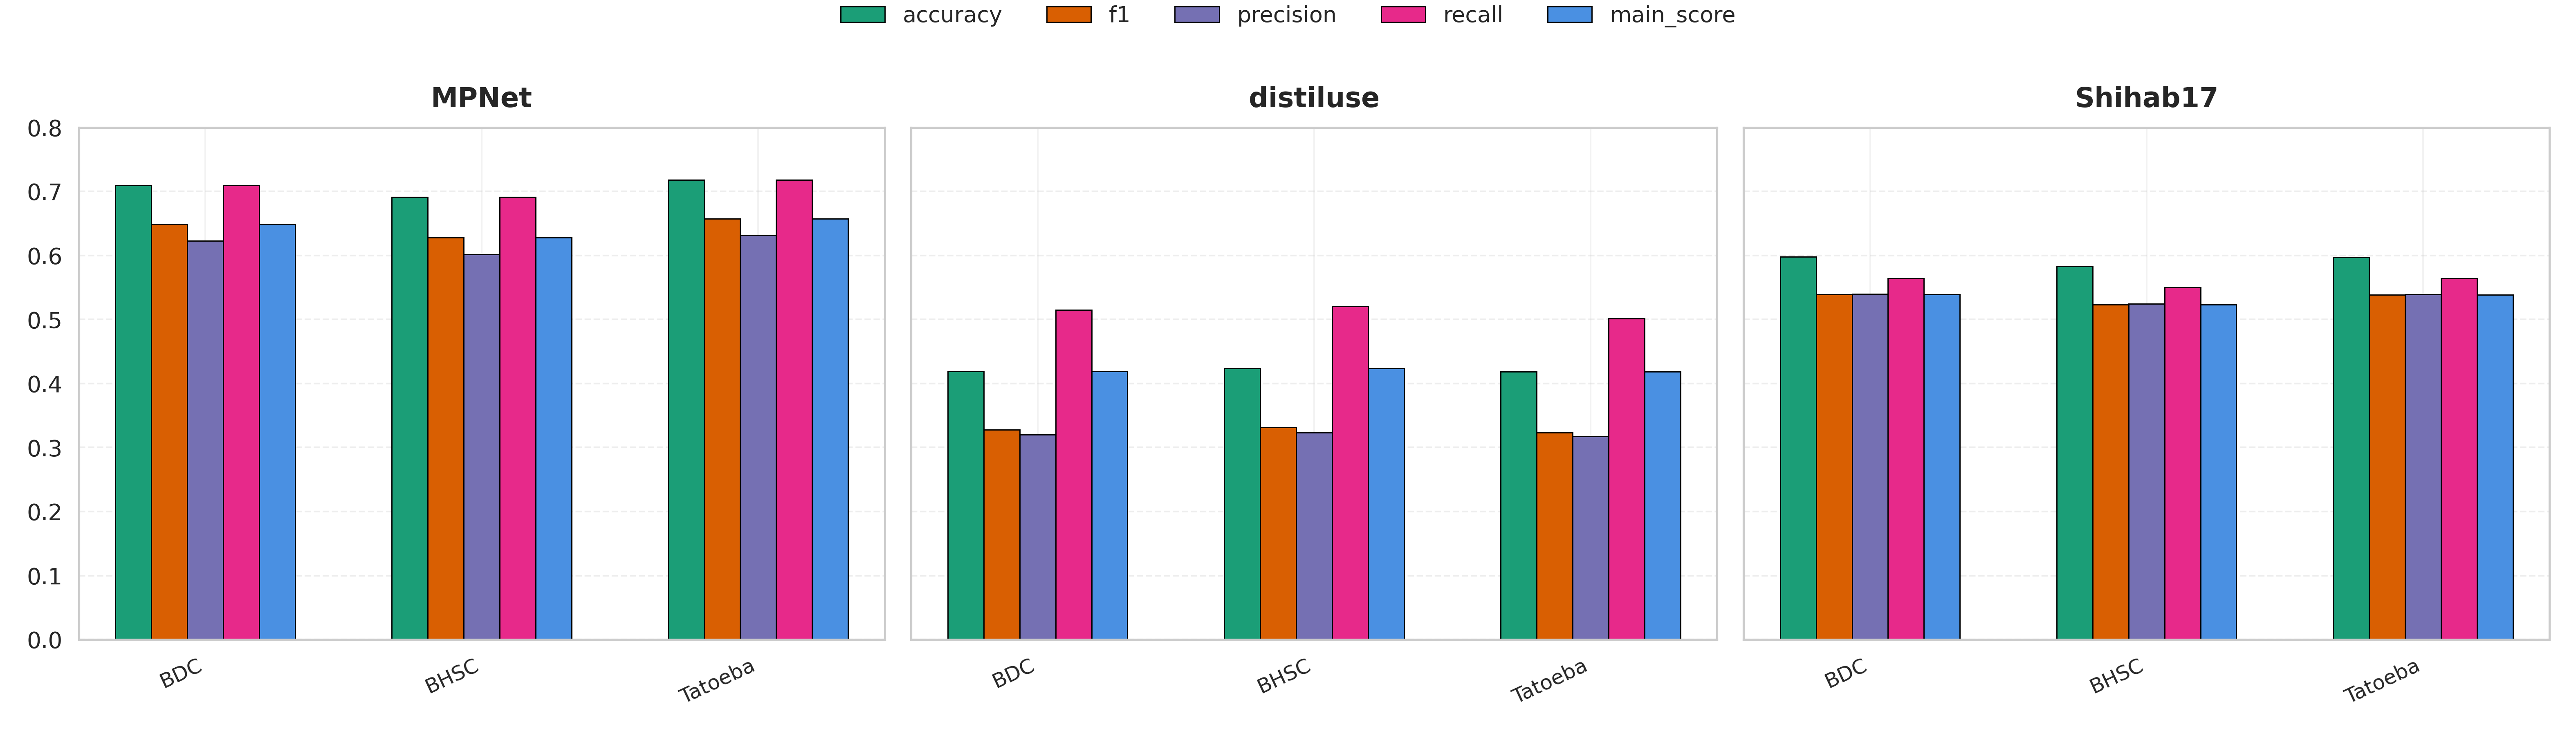
\includegraphics[width=\textwidth]{model_performance.png}
    \caption{Comparative performance on MTEB benchmark tasks, broken down by model. Each subplot shows a model's performance on Bengali Document Classification (BDC), Bengali Hate Speech Classification (BHSC), and Tatoeba retrieval. The MPNet model demonstrates consistently superior scores across all tasks and metrics.}
    \label{fig:mteb_breakdown}
    \Description{A multi-panel bar chart with three subplots side-by-side, one for each model: MPNet, distiluse, and Shihab17. Each subplot's x-axis lists the tasks (BDC, BHSC, Tatoeba) and the y-axis shows the score from 0.0 to 0.8. Within each task, five colored bars represent the metrics: accuracy, f1, precision, recall, and main_score. The bars in the MPNet subplot on the left are visibly higher than the corresponding bars in the distiluse and Shihab17 subplots, indicating superior performance.}
\end{figure*}


\section{Qualitative RAG Analysis}

To understand the downstream impact of these retrieval metrics, we integrated the fine-tuned models into a RAG pipeline. We utilized Radar Charts (Figure \ref{fig:radar}) to visualize the RAG metrics (Faithfulness, Answer Relevancy, Context Precision) comparing the low-resource (64d) and high-resource (512d) configurations.


\begin{xltabular}{\textwidth}{|p{2.5cm}|p{1.5cm}|p{5.5cm}|p{2.2cm}|p{1.2cm}|}
    \caption{Comparative RAG Responses: Success vs. Failure Cases}
    \label{tab:bengali_rag_examples} \\
    
    % --- Header for First Page ---
    \hline
    \textbf{Query} & \textbf{Model} & \textbf{Retrieved-Context} & \textbf{Generated Response} & \textbf{Result} \\
    \hline
    \endfirsthead
    
    % --- Header for Subsequent Pages ---
    \caption[]{Comparative RAG Responses (Continued)} \\
    \hline
    \textbf{Query} & \textbf{Model} & \textbf{Retrieved-Context} & \textbf{Generated Response} & \textbf{Result} \\
    \hline
    \endhead
    
    % --- Footer ---
    \hline
    \multicolumn{5}{r}{\textit{Continued on next page...}} \\
    \endfoot
    \hline
    \endlastfoot

    % ================= ROW 1 =================
    \bn{বিশ্বের প্রথম কম্পিউটার কে তৈরি করেন ?} \newline \textit{(Who created the first computer?)} 
    & mpnet-ft 
    & \scriptsize \bn{['১৮৩৭ খ্রীষ্টাব্দে চার্লস ব্যাবেজ একটি বিশ্লেষণধর্মী বা অ্যানালিটিকাল ইঞ্জিন-এর খসড়া তৈরী করেন যার মূল সুবিধাগুলি ছিল - এক্সপ্যান্ডেবেল মেমরি (বিস্তারযোগ্য যান্ত্রিক স্মৃতিশক্তি), গাণিতিক হিসাব করার ক্ষমতা, যুক্তিনির্ভর সিদ্ধান্ত নেওয়ার ক্ষমতা, লুপ ও কন্ডিশনাল ব্রাঞ্চিং(যা আধুনিক প্রোগ্রামিং ভাষাগুলিতে পাওয়া যায়) ইত্যাদি। এই যন্ত্রটিকে বিজ্ঞানীরা বিশ্বের প্রথম কম্পিউটার বলে স্বীকার করে থাকেন এবং ট্যুরিংসমতুল্য বলেও মনে করা হয়।', 'কম্পিউটারের গঠন ও প্রচলন নীতির ভিত্তিতে একে তিন ভাগে ভাগ করা যায়।', 'উইন্ডোজে ইউনিকোড ভিত্তিক বাংলা লেখার জন্য ২০০৩ সালের ২৬শে মার্চ অভ্র কীবোর্ড সফটওয়্যারটি আবির্ভূত হয়[1][2]। এটার সাহায্যে বাংলা লিপি ব্যবহার করে এমন সব ভাষাতেই টাইপ করা যায়। এ ধরনের ভাষার মধ্যে অসমীয়া ভাষা অন্যতম। মেহদী হাসান খান নামে ময়মনসিংহ মেডিকেল কলেজের একজন ছাত্র ২০০৩ সালে অভ্র কীবোর্ড তৈরির কাজ শুরু করেন। তিনি এটি সর্বপ্রথম তৈরি করেছিলেন ভিজুয়াল বেসিক প্রোগ্রামিং ভাষা দিয়ে, পরবর্তীতে তিনি তা ডেলফিতে ভাষান্তর করেন। এই সফটওয়্যারটির লিনাক্স সংস্করণ লেখা হয়েছে সি++ প্রোগ্রামিং']}
    & \bn{বিশ্বের প্রথম কম্পিউটার চার্লস ব্যাবেজ তৈরি করেন।} & \textbf{Success} \\
    \hline

    % ================= ROW 2 =================
    \bn{বিশ্বের প্রথম কম্পিউটার কে তৈরি করেন ?} \newline \textit{(Who created the first computer?)} 
    & distiluse-ft 
    & \scriptsize \bn{['কম্পিউটারের গঠন ও প্রচলন নীতির ভিত্তিতে একে তিন ভাগে ভাগ করা যায়।', '‘লুমিয়ের সিনেমাটোগ্রাফ’-এর মত বিশ্বব্যাপী প্রভাব বিস্তার করতে পারেনি। এই ঘটনার পরে পরেই সারা বিশ্ব জুড়ে প্রচুর ফিল্ম প্রোডাকশন কোম্পানি তৈরী হয়ে যায় আর মাত্র এক দশকের মধ্যেই চলচ্চিত্র তার অভিনবত্ত্ব কাটিয়ে উঠে এক বিশাল সর্বজনীন বিনোদনশিল্পে পরিণত হয়।', 'লিনাক্স সংস্করণ লেখা হয়েছে সি++ প্রোগ্রামিং ভাষায়। পরবর্তীতে রিফাত-উন-নবী, তানবিন ইসলাম সিয়াম, রাইয়ান কামাল, শাবাব মুস্তফা, ওমর ওসমান, সারিম খান এবং নিপুন হক এই সফটওয়্যারের উন্নয়নের সাথে যুক্ত হন।[1][3]']}
    & \bn{আমি জানি না।} & Failure \\
    \hline

    % ================= ROW 3 =================
    \bn{ঔপন্যাসিক ও গল্পকার জহির রায়হান পরিচালিত প্রথম চলচ্চিত্রের নাম কী ?} \newline \textit{(Name of first film by Jahir Raihan?)} 
    & mpnet-ft 
    & \scriptsize \bn{['জহির রায়হান বাংলা সাহিত্যে স্নাতকোত্তর ডিগ্রি লাভ করেন। তার সাহিত্যিক ও সাংবাদিক জীবন শুরু হয়। ১৯৫০ সালে তিনি যুগের আলো পত্রিকায় সাংবাদিক হিসেবে কাজ করা শুরু করেন। পরবর্তীতে তিনি খাপছাড়া, যান্ত্রিক, সিনেমা ইত্যাদি পত্রিকাতেও কাজ করেন। ১৯৫৬ সালে তিনি সম্পাদক হিসেবে প্রবাহ পত্রিকায় যোগ দেন। ১৯৫৫ সালে তার প্রথম গল্পগ্রন্থ সূর্যগ্রহণ প্রকাশিত হয়। চলচ্চিত্র জগতে তার পদার্পণ ঘটে ১৯৫৭ সালে, জাগো হুয়া সাভেরা ছবিতে সহকারী হিসেবে কাজ করার মাধ্যমে। তিনি সালাউদ্দীনের ছবি যে নদী মরুপথে</i>তেও সহকারী', 'তিনি সালাউদ্দীনের ছবি যে নদী মরুপথে</i>তেও সহকারী হিসেবে কাজ করেন। প্রখ্যাত চলচ্চিত্র পরিচালক এহতেশাম তাকে এ দেশ তোমার আমার এ কাজ করার আমন্ত্রণ জানান; জহির এ ছবির নামসঙ্গীত রচনা করেছিলেন। ১৯৬১ সালে তিনি রূপালী জগতে পরিচালক হিসেবে আত্মপ্রকাশ করেন কখনো আসেনি চলচ্চিত্রের মাধ্যমে। ১৯৬৪ সালে তিনি পাকিস্তানের প্রথম রঙিন চলচ্চিত্র সঙ্গম নির্মাণ করেন (উর্দু ভাষার ছবি) এবং পরের বছর তার প্রথম সিনেমাস্কোপ চলচ্চিত্র বাহানা মুক্তি দেন। জহির রায়হান ভাষা আন্দোলনে সক্রিয়ভাবে যুক্ত ছিলেন এবং ২১শে ফেব্রুয়ারির', 'বেশ কয়েকটি প্রদর্শনী হয় এবং চলচ্চিত্রটি দেখে সত্যজিত রায়, মৃণাল সেন, তপন সিনহা এবং ঋত্বিক ঘটক প্রমুখ ভূয়সী প্রশংসা করেন। সে সময়ে তিনি চরম অর্থনৈতিক দৈন্যের মধ্যে থাকা সত্ত্বেও তার চলচ্চিত্র প্রদর্শনী হতে প্রাপ্ত সমুদয় অর্থ তিনি মুক্তিযোদ্ধা তহবিলে দান করে দেন।[2]']}
    & \bn{জহির রায়হান পরিচালিত প্রথম চলচ্চিত্রের নাম "কখনো আসেনি"} & \textbf{Success} \\
    \hline

    % ================= ROW 4 =================
    \bn{ঔপন্যাসিক ও গল্পকার জহির রায়হান পরিচালিত প্রথম চলচ্চিত্রের নাম কী ?} \newline \textit{(Name of first film by Jahir Raihan?)} 
    & shihab17-ft 
    & \scriptsize \bn{[\'জহির রায়হান বাংলা সাহিত্যে স্নাতকোত্তর ডিগ্রি লাভ করেন। তার সাহিত্যিক ও সাংবাদিক জীবন শুরু হয়। ১৯৫০ সালে তিনি যুগের আলো পত্রিকায় সাংবাদিক হিসেবে কাজ করা শুরু করেন। পরবর্তীতে তিনি খাপছাড়া, যান্ত্রিক, সিনেমা ইত্যাদি পত্রিকাতেও কাজ করেন। ১৯৫৬ সালে তিনি সম্পাদক হিসেবে প্রবাহ পত্রিকায় যোগ দেন। ১৯৫৫ সালে তার প্রথম গল্পগ্রন্থ সূর্যগ্রহণ প্রকাশিত হয়। চলচ্চিত্র জগতে তার পদার্পণ ঘটে ১৯৫৭ সালে, জাগো হুয়া সাভেরা ছবিতে সহকারী হিসেবে কাজ করার মাধ্যমে। তিনি সালাউদ্দীনের ছবি যে নদী মরুপথে</i>তেও সহকারী\', \'দেবশ্রী রায় এর জন্ম, বেড়ে ওঠা কলকাতায়। তার পিতার নাম বীরেন্দ্র কিশোর রায় এবং মায়ের নাম আরতি রায়। ১৯৬৯ সনে তিনি প্রথম "বালক গদাধর" নামে একটি চলচিত্রে শিশুশিল্পী হিসেবে অভিনয় করেন, যার পরিচালক ছিলেন হরিময় সেন। তিনি কলকাতার এ পি জে ,পার্ক স্ট্রীট শাখার স্কুলের ছাত্রী ছিলেন, যদিও নাচের প্রতি অত্যধিক ঝোঁক থাকার কারণে বেশিদূর এগোতে পারেন নি। তার ডাক নাম চুমকি।\', \'বেশ কয়েকটি প্রদর্শনী হয় এবং চলচ্চিত্রটি দেখে সত্যজিত রায়, মৃণাল সেন, তপন সিনহা এবং ঋত্বিক ঘটক প্রমুখ ভূয়সী প্রশংসা করেন। সে সময়ে তিনি চরম অর্থনৈতিক দৈন্যের মধ্যে থাকা সত্ত্বেও তার চলচ্চিত্র প্রদর্শনী হতে প্রাপ্ত সমুদয় অর্থ তিনি মুক্তিযোদ্ধা তহবিলে দান করে দেন।[2]\']}
    & \bn{আমি জানি না।} & Failure \\
    \hline

    % ================= ROW 5 =================
    \bn{ভারতের ছত্তীসগঢ় রাজ্যের রাজধানী কোথায় ?} \newline \textit{(Where is the capital of Chhattisgarh?)}
    & mpnet-ft 
    & \scriptsize \bn{[\'ছত্তীসগঢ় (ছত্তীসগঢ়ি/হিন্দি: মধ্য ভারতের একটি রাজ্য। ২০০১ সালের ১ নভেম্বর মধ্যপ্রদেশ রাজ্যের দক্ষিণ-পশ্চিমাঞ্চলে স্থিত ষোলোটি ছত্তীসগঢ়ি-ভাষী জেলা নিয়ে এই রাজ্য স্থাপন করা হয়। রায়পুর এই রাজ্যের রাজধানী। ৫২,১৯৯ বর্গমাইল (১৩৫,১৯৪ বর্গকিলোমিটার) আয়তন বিশিষ্ট এই রাজ্য ভারতের দশম বৃহত্তম রাজ্য।\', \'দেবশ্রী রায় এর জন্ম, বেড়ে ওঠা কলকাতায়। তার পিতার নাম বীরেন্দ্র কিশোর রায় এবং মায়ের নাম আরতি রায়। ১৯৬৯ সনে তিনি প্রথম "বালক গদাধর" নামে একটি চলচিত্রে শিশুশিল্পী হিসেবে অভিনয় করেন, যার পরিচালক ছিলেন হরিময় সেন। তিনি কলকাতার এ পি জে ,পার্ক স্ট্রীট শাখার স্কুলের ছাত্রী ছিলেন, যদিও নাচের প্রতি অত্যধিক ঝোঁক থাকার কারণে বেশিদূর এগোতে পারেন নি। তার ডাক নাম চুমকি।\', \'জমিদারি নিলামে ক্রয় করেন। তাঁর জমিদারিতে বেশ কিছু অংশীদার ও সহ-অংশীদার ছিলেন। কিন্তু তিনি বহরমপুর, পাণ্ডুয়া, কালীগ্রাম ও শাহজাদপুরে চারটি বড় জমিদারির মালিক ছিলেন এবং এগুলিতে তাঁর কোন অংশীদার ছিল না। ১৮৪০ সালে সেগুলি তিনি তাঁর সন্তান ও তাঁদের উত্তরাধিকারীদের ট্রাস্ট করে দেন। দ্বারকানাথ ঠাকুরের জমিদারি পরিচালনার একটি বিশেষ বৈশিষ্ট্য ছিল। তিনি এটিকে সামন্ততন্ত্রের দৃষ্টিকোণ থেকে না দেখে মূলধনের সৃষ্টিশীল প্রসার হিসেবে বিবেচনা করেন। এক্ষেত্রে তিনি সমকালীন জমিদারদের চেয়ে ব্যতিক্রম ছিলেন। জমিদারি\']}
    & \bn{রায়পুর।} & \textbf{Success} \\
    \hline

    % ================= ROW 6 =================
    \bn{ভারতের ছত্তীসগঢ় রাজ্যের রাজধানী কোথায় ?} \newline \textit{(Where is the capital of Chhattisgarh?)}
    & distiluse-ft 
    & \scriptsize \bn{[\'ছত্তীসগঢ় (ছত্তীসগঢ়ি/হিন্দি: মধ্য ভারতের একটি রাজ্য। ২০০১ সালের ১ নভেম্বর মধ্যপ্রদেশ রাজ্যের দক্ষিণ-পশ্চিমাঞ্চলে স্থিত ষোলোটি ছত্তীসগঢ়ি-ভাষী জেলা নিয়ে এই রাজ্য স্থাপন করা হয়। রায়পুর এই রাজ্যের রাজধানী। ৫২,১৯৯ বর্গমাইল (১৩৫,১৯৪ বর্গকিলোমিটার) আয়তন বিশিষ্ট এই রাজ্য ভারতের দশম বৃহত্তম রাজ্য।\', \'দেবশ্রী রায় এর জন্ম, বেড়ে ওঠা কলকাতায়। তার পিতার নাম বীরেন্দ্র কিশোর রায় এবং মায়ের নাম আরতি রায়। ১৯৬৯ সনে তিনি প্রথম "বালক গদাধর" নামে একটি চলচিত্রে শিশুশিল্পী হিসেবে অভিনয় করেন, যার পরিচালক ছিলেন হরিময় সেন। তিনি কলকাতার এ পি জে ,পার্ক স্ট্রীট শাখার স্কুলের ছাত্রী ছিলেন, যদিও নাচের প্রতি অত্যধিক ঝোঁক থাকার কারণে বেশিদূর এগোতে পারেন নি। তার ডাক নাম চুমকি।\', \'গণচীন সরকারের ১৯৫১ খ্রিষ্টাব্দে স্বাক্ষরিত চুক্তিকে বোঝানো হয়, যার ফলে তিব্বত গণচীনের অধীনে একটি স্বয়ংশাসিত অঞ্চলে পরিণত হয়।\']}
    & \bn{রায়পুর।} & \textbf{Success} \\
    \hline

\end{xltabular}

\begin{figure*}[ht!]
    \centering
    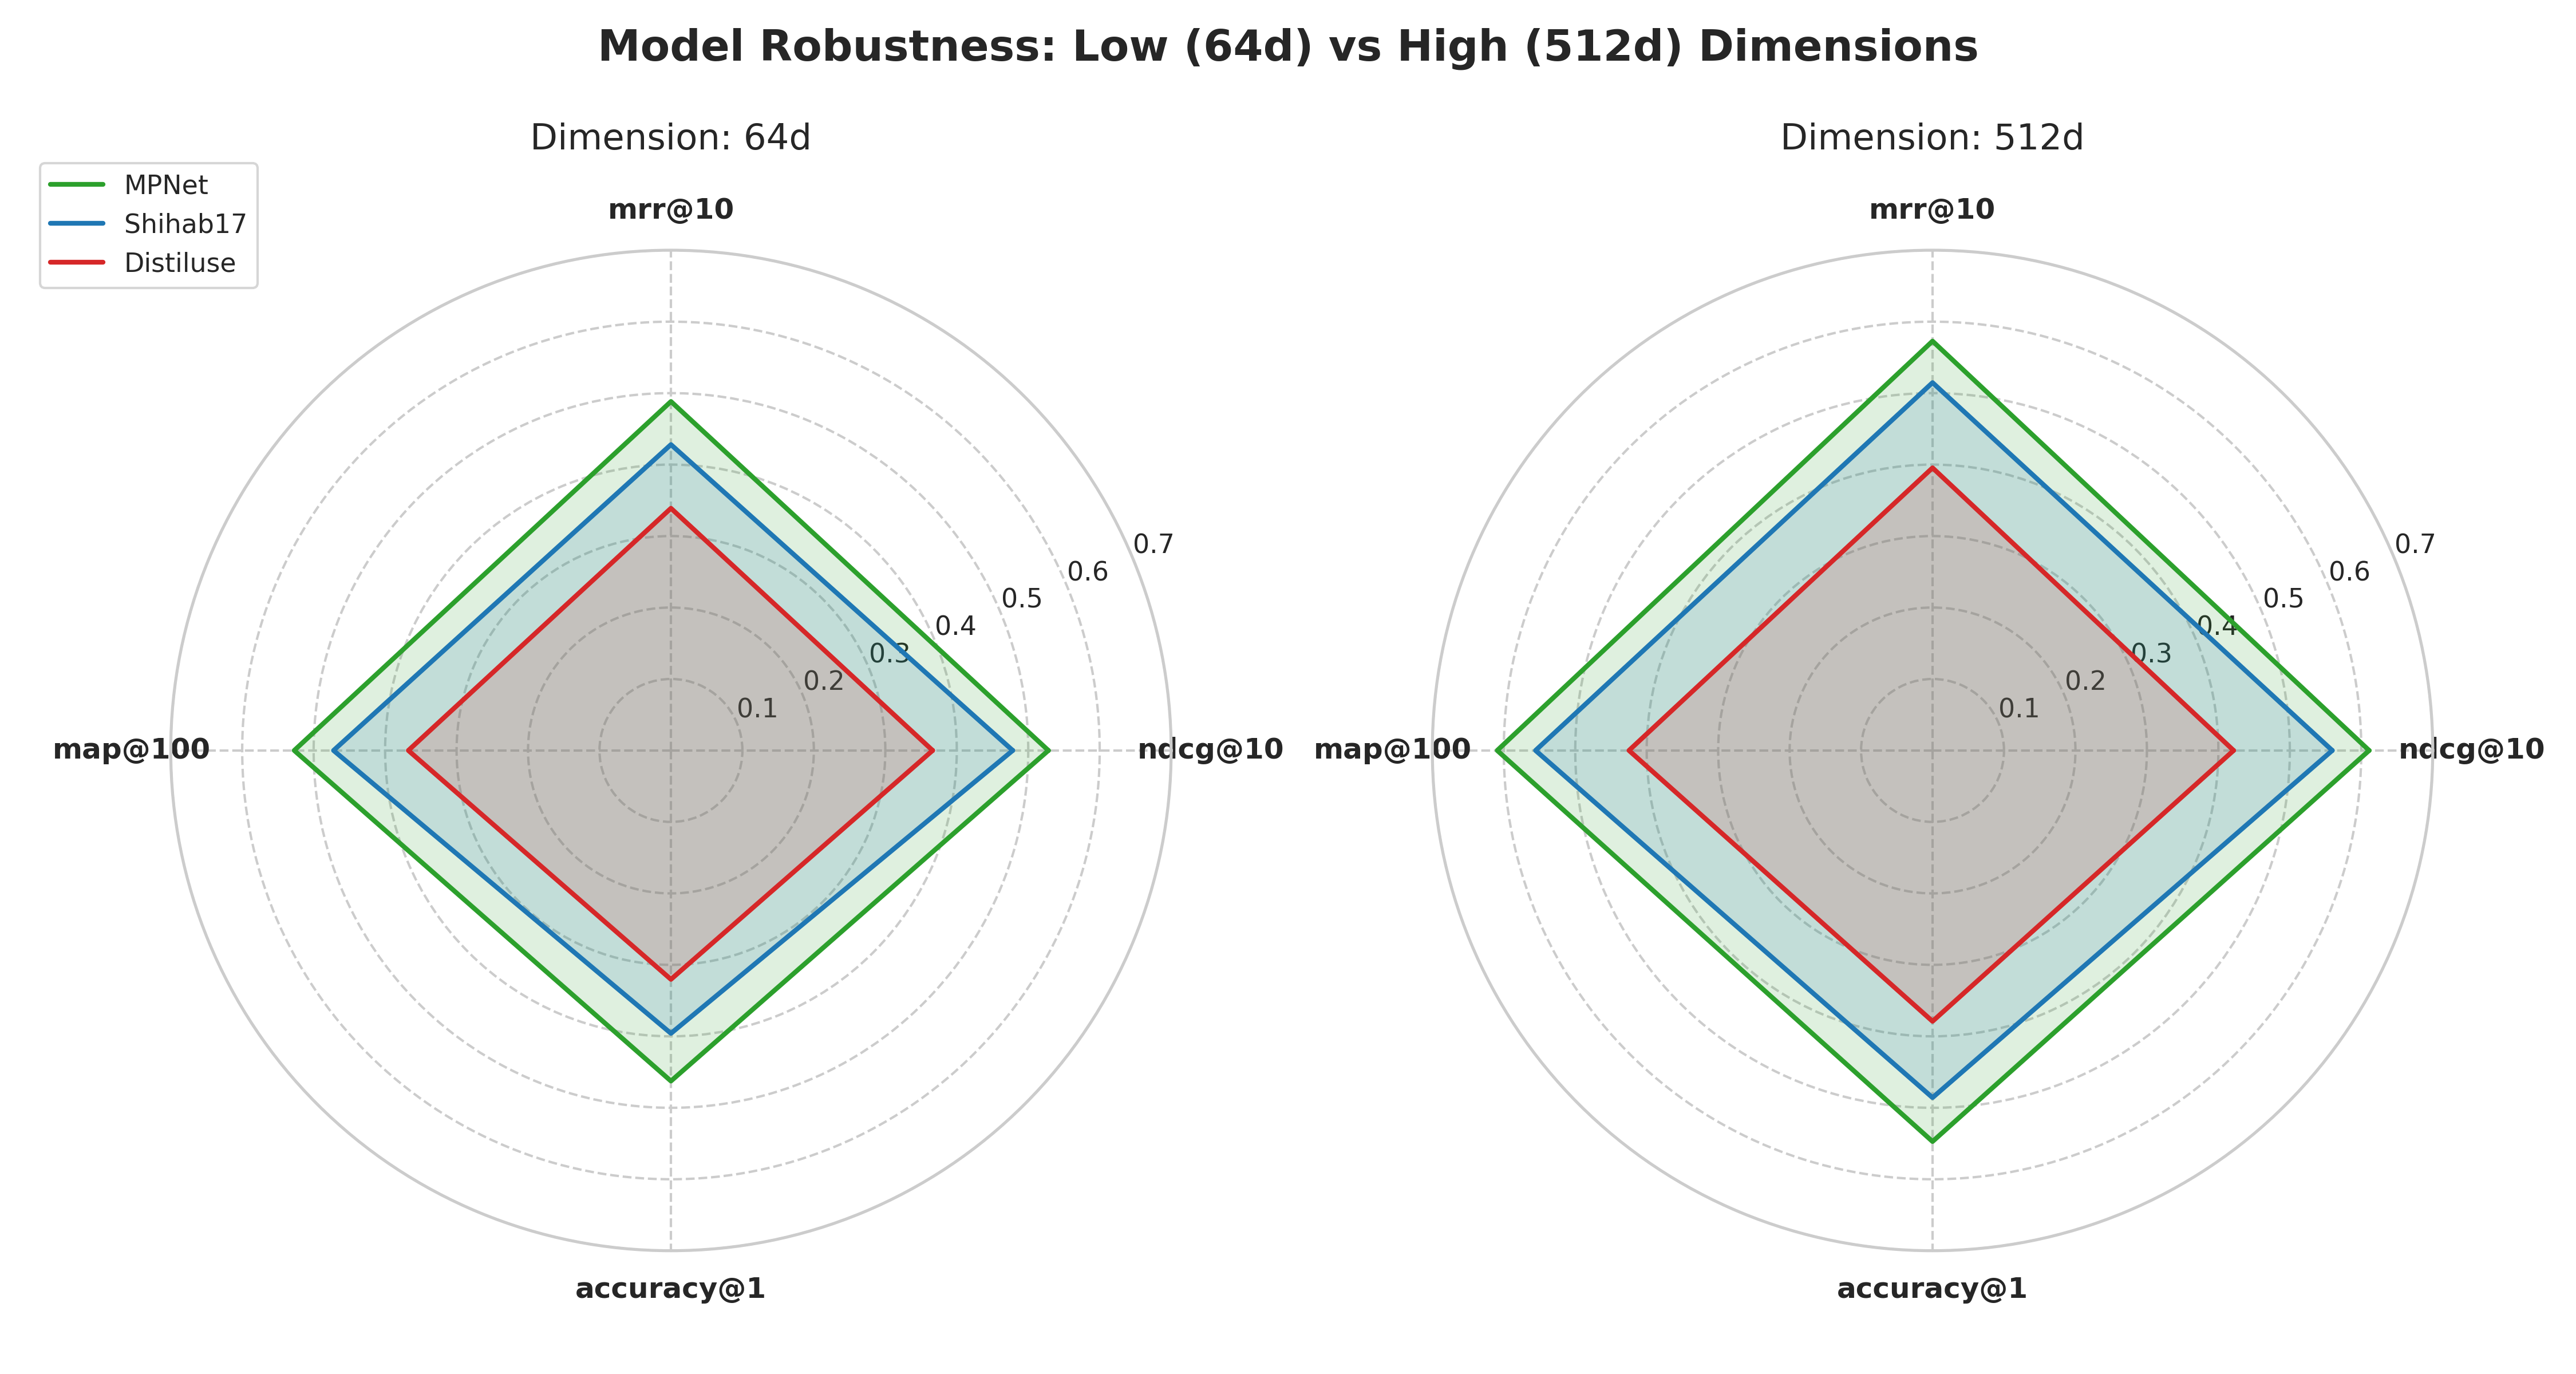
\includegraphics[width=0.9\textwidth]{paper_plot_radar_chart.png}
    \caption{Radar charts comparing model robustness at Low (64d) vs High (512d) dimensions. Even at extreme compression (64d), the MPNet model (green area) covers a larger surface area across metrics than the full-precision Distiluse model.}
    \label{fig:radar}
    \Description{Two radar charts side-by-side. The left chart shows performance at 64 dimensions, the right at 512 dimensions. The axes are Faithfulness, Answer Relevancy, and Context Precision. The green shaded area (MPNet) is larger than the other colored areas in both charts.}
\end{figure*}



\subsection{Operational Efficiency and Storage Costs}

For real-world deployment, specifically in Retrieval-Augmented Generation (RAG) systems where vector database costs scale linearly with dimensionality, the trade-off between storage footprint and retrieval accuracy is paramount. We analyzed this trade-off by comparing the physical storage requirements against NDCG@10 scores across varying dimensions on our test corpus of 1,124 documents.

Figure~\ref{fig:efficiency} illustrates the Pareto frontier of efficiency. The fine-tuned \texttt{mpnet} model demonstrates remarkable resilience to quantization. As detailed in Table~\ref{tab:efficiency}, reducing the dimensionality from $768d$ to $128d$ results in an $83.3\%$ reduction in memory usage (dropping from 3.29 MB to 0.55 MB). Despite this massive compression, the model retains $96.1\%$ of its peak performance ($0.7796$ vs $0.8114$ NDCG).

Crucially, even at the extreme compression of $64d$, the fine-tuned MPNet achieves an NDCG of $0.7438$, which is significantly higher than the full-precision ($768d$) performance of the original pre-trained base model ($0.4715$). This confirms that our Matryoshka fine-tuning strategy not only aligns the vector space for Bengali but does so in a way that concentrates semantic information into the earlier dimensions, identifying $128d$ as the ideal configuration for resource-constrained production environments.


\begin{figure}[htbp]
    \centering
    % Ensure the filename matches what you saved in Colab
    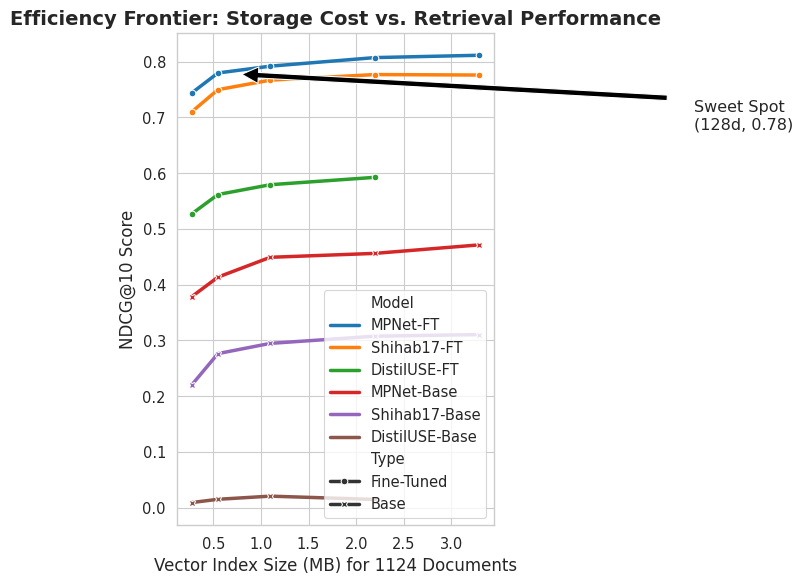
\includegraphics[width=0.95\linewidth]{efficiency-tradeoff.png}
    \caption{\textbf{The Efficiency-Accuracy Trade-off.} The X-axis represents the memory footprint (MB) required to index the test corpus ($N=1124$), while the Y-axis shows retrieval performance (NDCG@10). The fine-tuned \texttt{mpnet-ft} model (blue line) exhibits a superior performance curve. The annotation highlights the operational ``sweet spot'' at 128 dimensions, offering high accuracy with an $83\%$ reduction in storage costs compared to the 768d baseline.}
    \label{fig:efficiency}
\end{figure}


\begin{table}[h]
    \centering
    \caption{Storage vs. Performance Analysis. Comparison of the Base model against the Fine-Tuned (FT) MPNet model across compression levels. At 128d, the model retains 96\% of its performance while reducing storage by $83\%$.}
    \label{tab:efficiency}
    \begin{tabular}{lcccc}
        \toprule
        \textbf{Model Config.} & \textbf{Dim.} & \textbf{Size (MB)} & \textbf{NDCG@10} & \textbf{Retention} \\
        \midrule
        MPNet-Base & 768d & 3.29 MB & 0.4715 & - \\
        \textbf{MPNet-FT} & \textbf{768d} & 3.29 MB & \textbf{0.8114} & \textbf{100.0\%} \\
        \midrule
        \textit{Compression Analysis} & & & & \\
        MPNet-FT & 512d & 2.20 MB & 0.8072 & 99.5\% \\
        MPNet-FT & 256d & 1.10 MB & 0.7918 & 97.6\% \\
        \textbf{MPNet-FT} & \textbf{128d} & \textbf{0.55 MB} & \textbf{0.7796} & \textbf{96.1\%} \\
        MPNet-FT & 64d & 0.27 MB & 0.7438 & 91.7\% \\
        \bottomrule
    \end{tabular}
\end{table}

\subsection{Response Accuracy and Hallucination}
The analysis reveals that MPNet's superior retrieval metrics translate directly to better generation. As shown in Figure \ref{fig:radar}, the MPNet profile (green) encompasses the others even at 64 dimensions.

Consider the query: \textit{"Who was the director of the world's first film?"}
\begin{itemize}
    \item The \texttt{shihab17} and \texttt{distiluse} models failed to retrieve the correct paragraph regarding the Lumière brothers. Consequently, the generation component hallucinated.
    \item The \texttt{mpnet} model correctly identified that the information was missing and responded with "I don't know," resulting in a high Faithfulness score.
\end{itemize}

Figure \ref{fig:heatmap} further correlates model confidence with retrieval success, indicating that \texttt{mpnet} embeddings are more semantically precise, effectively distinguishing between topical relevance and factual answers.

\begin{figure}[ht!]
    \centering
    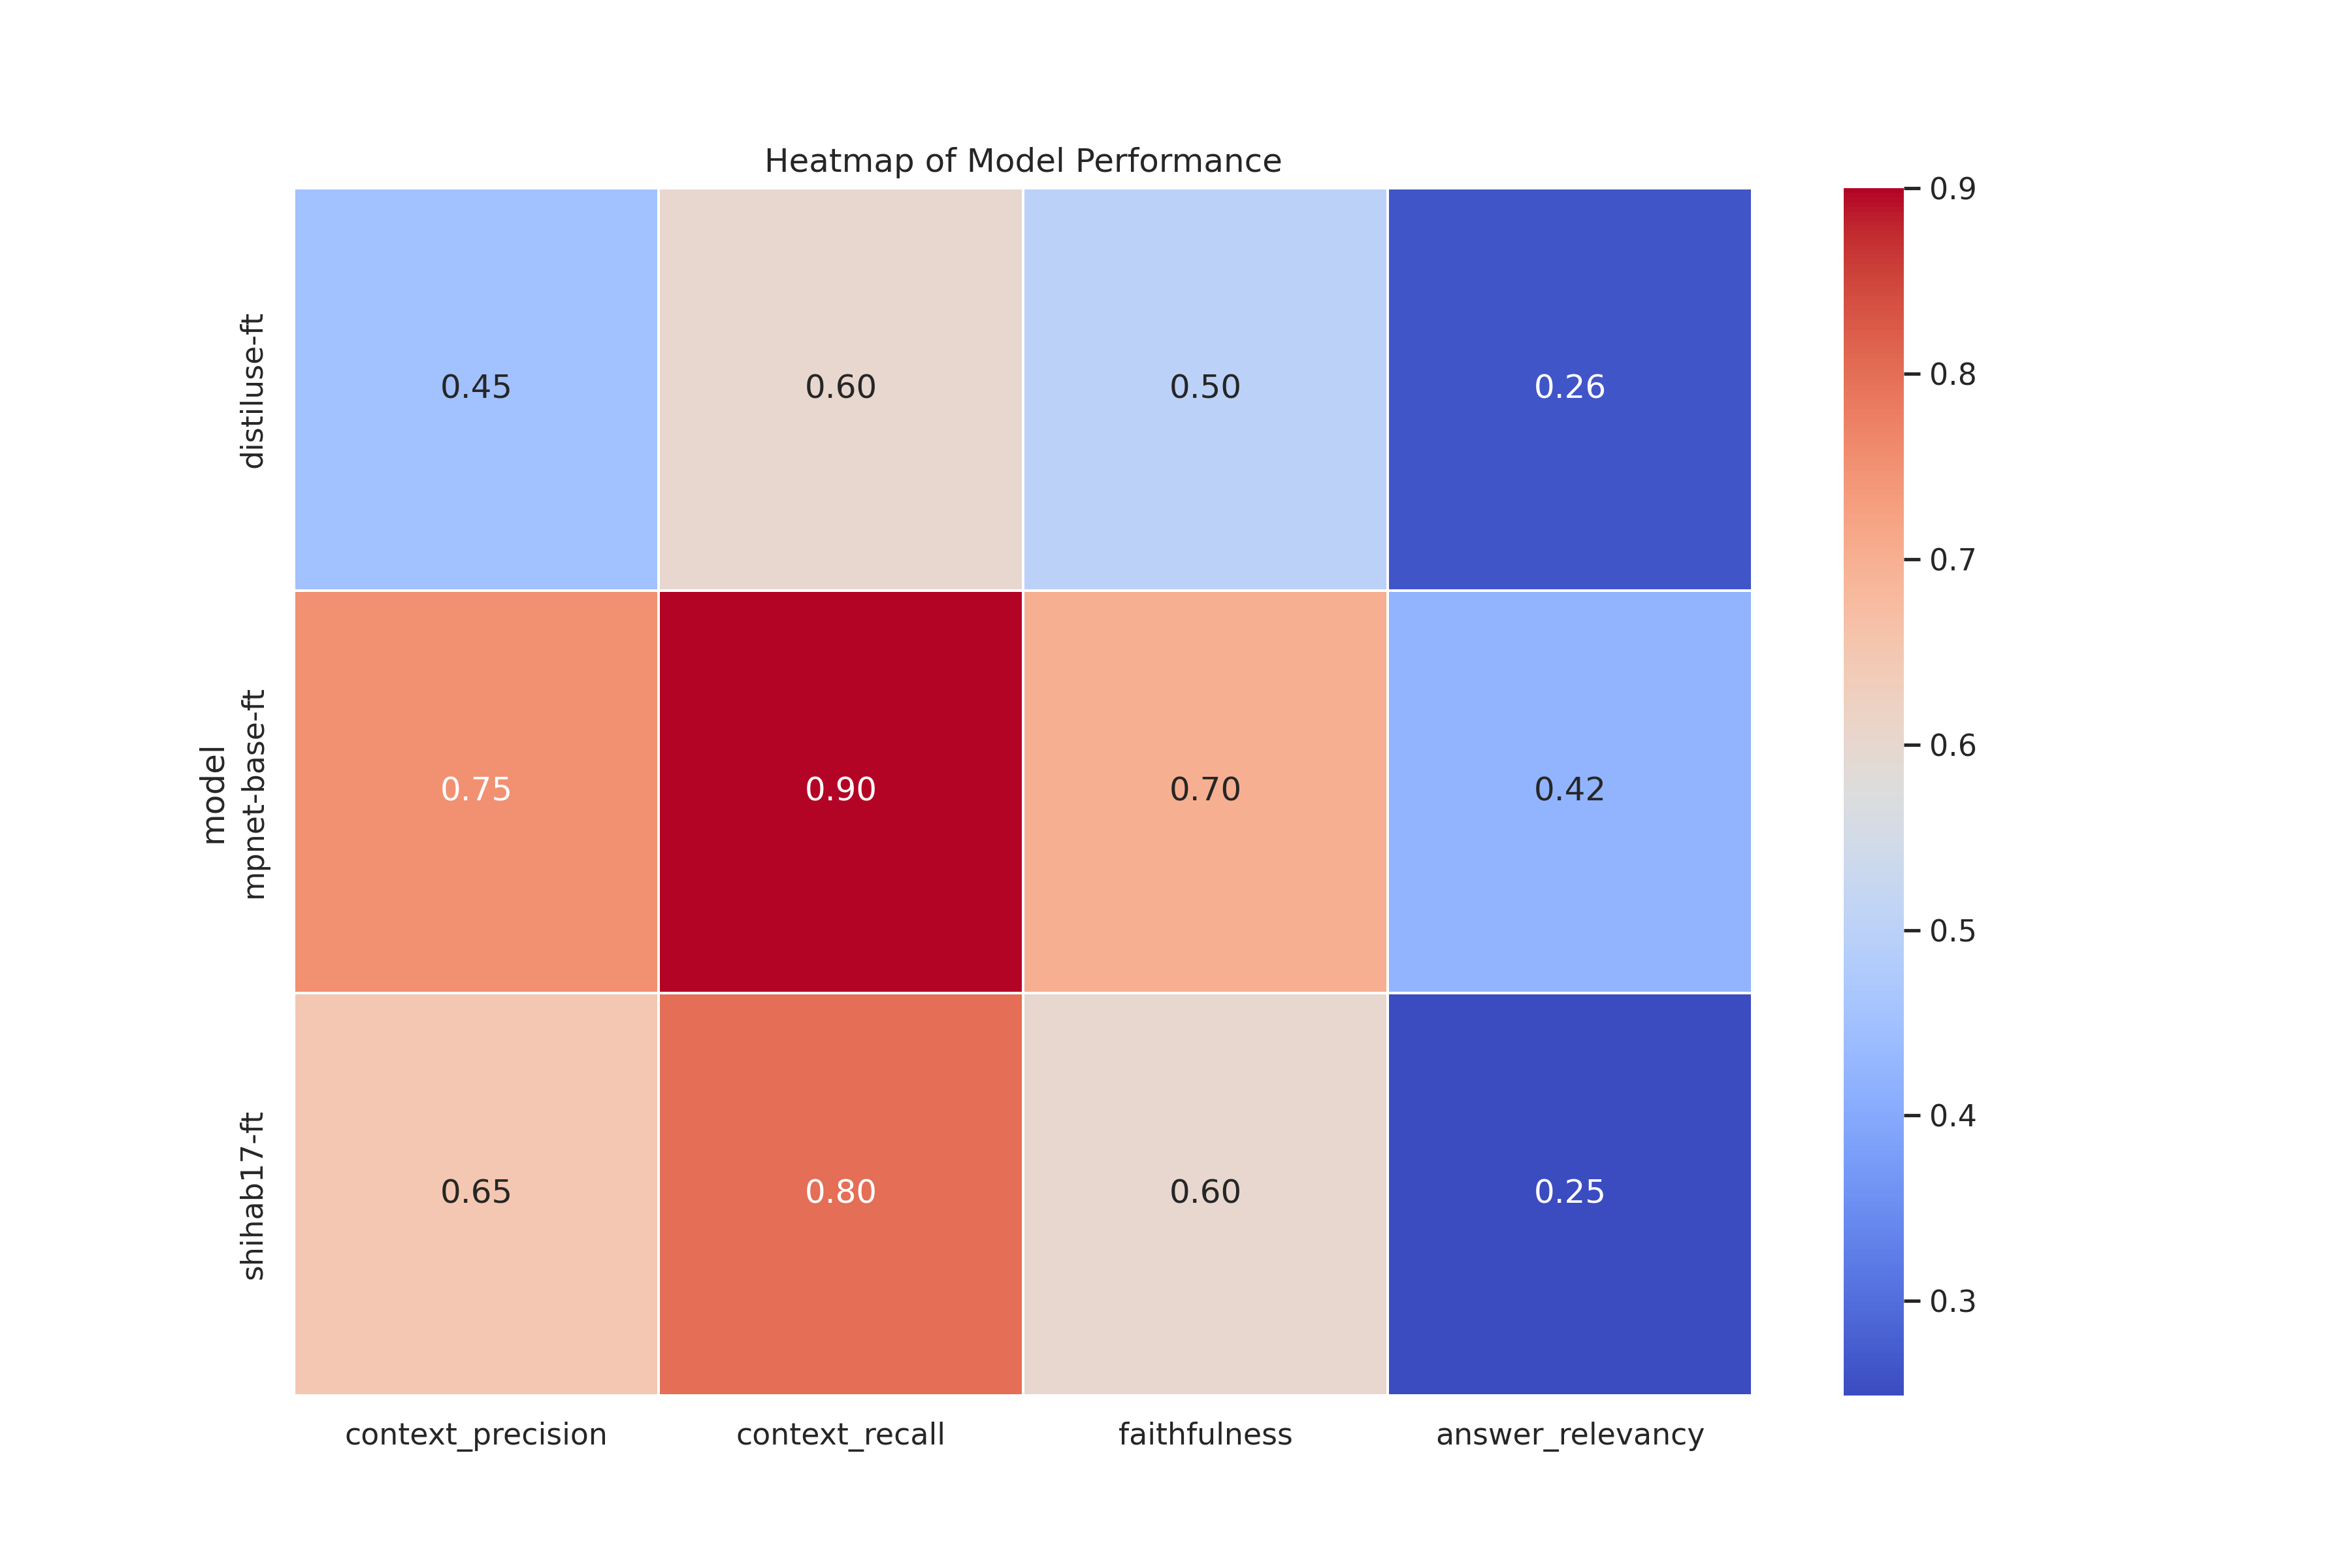
\includegraphics[width=\linewidth]{heatmap.png}
    \caption{Heatmap illustrating the correlation between retrieval confidence and generation accuracy across different query types.}
    \label{fig:heatmap}
    \Description{A heatmap where colors represent correlation strength. One axis lists query types, the other lists confidence/accuracy metrics. High correlation is visible for MPNet.}
\end{figure}


\subsection{Error Analysis and Model Limitations}

While the quantitative metrics highlight \texttt{mpnet-ft} as the superior model, a granular analysis of failure cases reveals distinct behavioral patterns intrinsic to each architecture. We categorized 100 error samples from the test set into three primary failure modes: \textit{Lexical Overlap Bias}, \textit{Entity Hallucination}, and \textit{Tokenization Granularity}.

\textbf{Lexical Overlap Bias:} The distilled model (\texttt{distiluse}) frequently succumbed to lexical overlap bias, retrieving contexts that shared high keyword frequency with the query but lacked semantic alignment. For example, for the query \textit{"What is the currency of Bangladesh?"}, \texttt{distiluse} retrieved passages discussing "Bangladesh's economic growth" rather than the specific currency entity. In contrast, \texttt{mpnet}, with its deeper interaction layers, successfully mapped the query to contexts containing the specific answer "Taka", even when the word overlap was lower.

\textbf{Tokenization and Monolingual Advantage:} Although \texttt{mpnet} dominated overall, the monolingual \texttt{shihab17} model exhibited superior performance on queries involving rare Bengali idioms or complex agglutinative morphology.
Table~\ref{tab:error_analysis} illustrates a specific case where \texttt{mpnet} failed. The compound word \bn{‘মুক্তিযুদ্ধভিত্তিক’} (Liberation War-based) was split into four sub-tokens by the multilingual tokenizer of MPNet, diluting its semantic representation. The monolingual tokenizer of \texttt{shihab17} treated it as a more cohesive unit, allowing it to retrieve the correct literary context.

\textbf{False Negatives in High Compression:} At extreme compression (64d), \texttt{mpnet} occasionally failed to distinguish between negation and affirmation. In queries asking \textit{"Which feature is NOT present in..."}, the 64-dimensional vector lost the specific dimension encoding the negation, retrieving positive instances instead. This suggests that while Matryoshka learning is efficient, syntactic nuances like negation require higher dimensional bandwidth (minimum 128d).

\begin{table}[h]
    \caption{Error Analysis: Instance where Monolingual Model outperforms MPNet due to Tokenization}
    \label{tab:error_analysis}
    \small
    \begin{tabularx}{\linewidth}{p{1.5cm}X}
        \toprule
        \textbf{Query} & \bn{মুক্তিযুদ্ধভিত্তিক উপন্যাসের নাম কী?} \\
        \textit{(Trans.)} & \textit{What is the name of the Liberation War-based novel?} \\
        \midrule
        \textbf{Correct Context} & ...\bn{আনোয়ার পাশা রচিত 'রাইফেল রোটি আওরাত' একটি উল্লেখযোগ্য মুক্তিযুদ্ধভিত্তিক উপন্যাস।...} \\
        \midrule
        \textbf{MPNet-FT} & \textbf{Failure:} Retrieved a passage about general Bengali literature history. \\
        \textit{(Reason)} & Tokenizer fragmentation of \bn{‘মুক্তিযুদ্ধভিত্তিক’} resulted in loss of specific "war" context. \\
        \midrule
        \textbf{Shihab17-FT} & \textbf{Success:} Correctly retrieved the passage regarding 'Rifle Roti Aurat'. \\
        \textit{(Reason)} & Optimized Bengali vocabulary retained the compound word semantics. \\
        \bottomrule
    \end{tabularx}
\end{table}


\section{Limitations}

While our results are promising, this study has several limitations. First, our fine-tuning and evaluation are restricted to the \textit{BanglaRQA} dataset, which primarily consists of factoid questions from Wikipedia. The models' performance on conversational queries, abstract reasoning, or domain-specific texts (e.g., medical or legal Bengali) remains untested. 

Second, while we demonstrate the efficiency of Matryoshka Representation Learning, we did not perform an ablation study to quantify the specific contribution of the MRL objective versus the Multiple Negatives Ranking Loss alone. 

Finally, our error analysis indicates that while \texttt{mpnet} is superior, it still struggles with negation and complex morphological compounds at high compression rates (64d), suggesting that a minimum dimensionality of 128d is a hard constraint for semantic nuance.


\section{Ethics Statement}

This work utilizes the publicly available BanglaRQA dataset, derived from Wikipedia, which does not contain personally identifiable information (PII) or offensive content. Our models are intended to improve information access for Bengali speakers. However, we acknowledge that retrieval models can inadvertently surface biased or hallucinated content if the underlying knowledge base is flawed. All models and code will be released open-source to promote transparency. Regarding environmental impact, our experiments were conducted on a single GPU for less than one hour, resulting in a negligible carbon footprint compared to training Large Language Models from scratch.

\section{Conclusion}

This study provided a comparative evaluation of three distinct embedding architectures for Bengali semantic retrieval. Our results conclusively demonstrate that while specialized fine-tuning improves all models, the underlying architecture sets the performance ceiling. The \texttt{mpnet-base} model, when fine-tuned using our proposed Matryoshka-MNRL strategy, outperforms both the monolingual and distilled models. This finding holds true not only on our primary retrieval task but also across a range of classification and retrieval tasks from the MTEB benchmark.

We further demonstrated that high-dimensional embeddings are often unnecessary for effective retrieval in Bengali. Our saturation and retention analysis confirms that models can maintain over 95\% of their peak performance even when compressed to 128 dimensions. For practitioners building Bengali RAG applications, this suggests that the \texttt{mpnet} architecture, combined with dimensionality reduction, offers the optimal balance of accuracy and computational efficiency.

%%
%% The acknowledgments section is defined using the "acks" environment
%% (and NOT an unnumbered section).
\begin{acks}
The authors acknowledge the open-source contributions of the model creators for \texttt{shihab17/bangla-sentence-transformer}, \texttt{sentence-transformers}, and the curators of the BanglaRQA dataset.
\end{acks}

%%
%% The next two lines define the bibliography style to be used, and
%% the bibliography file.
% \begin{thebibliography}{99}

%     \bibitem{lewis2020retrieval}
%     P. Lewis, E. Perez, A. Piktus, et al. 2020. Retrieval-augmented generation for knowledge-intensive nlp tasks. In \emph{Advances in Neural Information Processing Systems} (NeurIPS).
    
%     \bibitem{gao2023survey}
%     Y. Gao, Y. Li, S. Yang, et al. 2023. Retrieval-Augmented Generation for Large Language Models: A Survey. \emph{arXiv preprint arXiv:2312.10997}.

%     \bibitem{hu2024comprehensive}
%     Z. Hu, Y. Chen, L. Wang, et al. 2024. A Comprehensive Survey of Retrieval-Augmented Generation (RAG). \emph{arXiv preprint arXiv:2407.03126}.

%     \bibitem{lin2024improving}
%     B. Y. Lin, A. Drozd, P. Budzianowski, et al. 2024. Improving Retrieval-Augmented Generation for Low-Resource Languages. In \emph{2024 IEEE International Conference on Acoustics, Speech, and Signal Processing (ICASSP)}.

%     \bibitem{debanath2025advancing}
%     K. Debanath, S. Aich, and A. Y. Srizon. 2025. Advancing Low-Resource NLP: Contextual Question Answering for Bengali Language Using Llama. In \emph{2025 International Conference on Electrical, Computer and Communication Engineering (ECCE)}.
    
%     \bibitem{yasunaga2022retrieval}
%     M. Yasunaga, J. Leskovec, P. Liang. 2022. Retrieval-Augmented Retrieval for Code Search and Completion. In \emph{Proceedings of the 60th Annual Meeting of the Association for Computational Linguistics (Volume 1: Long Papers)}.

%     \bibitem{conneau2019unsupervised}
%     A. Conneau, K. Khandelwal, N. Goyal, et al. 2019. Unsupervised cross-lingual representation learning at scale. \emph{arXiv preprint arXiv:1911.02116}.
    
%     \bibitem{ekram2022banglarqa}
%     S. M. S. Ekram, et al. 2022. BanglaRQA: A Benchmark Dataset for Under-resourced Bangla Language Reading Comprehension-based Question Answering. In \emph{Findings of the Association for Computational Linguistics: EMNLP 2022}.
    
%     \bibitem{kusupati2022matryoshka}
%     A. Kusupati, G. Bhatt, A. Rege, et al. 2022. Matryoshka representation learning. In \emph{Advances in Neural Information Processing Systems} (NeurIPS).
    
%     \bibitem{reimers2019sentence}
%     N. Reimers and I. Gurevych. 2019. Sentence-bert: Sentence embeddings using siamese bert-networks. In \emph{Proceedings of the 2019 Conference on Empirical Methods in Natural Language Processing and the 9th International Joint Conference on Natural Language Processing (EMNLP-IJCNLP)}.

%     \bibitem{bhattacharjee2020banglabert}
%     A. Bhattacharjee, et al. 2021. BanglaBERT: A Trivalent Perspective for Judging Bengali Language Models. \emph{arXiv preprint arXiv:2104.09633}.

%     \bibitem{uddin2024bangla}
%     M. S. Uddin, M. A. Haque, R. H. Rifat, et al. 2024. Bangla SBERT - Sentence Embedding Using Multilingual Knowledge Distillation. In \emph{2024 IEEE 15th Annual Ubiquitous Computing, Electronics \& Mobile Communication Conference (UEMCON)}.

%     \bibitem{reimers2019sentencebert}
%     Reimers, Nils and Gurevych, Iryna. 2019. Sentence-BERT: Sentence Embeddings using Siamese BERT-Networks. In \emph{2019 Conference on Empirical Methods in Natural Language Processing}


%     \bibitem{kabir2024banglaembed}
%     M. R. Kabir, M. M. R. Nabil, and M. A. Khan. 2024. BanglaEmbed: Efficient Sentence Embedding Models for a Low-Resource Language Using Cross-Lingual Distillation Techniques. In \emph{2024 6th International Conference on Advanced Information and Communication Technology (ICAICT)}.
    
%     \bibitem{song2020mpnet}
%     K. Song, X. Tan, T. Qin, J. Lu, and T.-Y. Liu. 2020. MPNet: Masked and Permuted Pre-training for Language Understanding. In \emph{Advances in Neural Information Processing Systems} (NeurIPS).
    
%     \bibitem{yang2019multilingual}
%     Y. Yang, et al. 2019. Multilingual Universal Sentence Encoder for Semantic Retrieval. In \emph{Proceedings of the 57th Annual Meeting of the Association for Computational Linguistics}.

% \end{thebibliography}

% \begin{thebibliography}{99}

%     \bibitem{lewis2020retrieval}
%     P. Lewis, E. Perez, A. Piktus, et al. 2020. Retrieval-augmented generation for knowledge-intensive nlp tasks. In \emph{Advances in Neural Information Processing Systems} (NeurIPS).
    
%     \bibitem{gao2023survey}
%     Y. Gao, Y. Li, S. Yang, et al. 2023. Retrieval-Augmented Generation for Large Language Models: A Survey. \emph{arXiv preprint arXiv:2312.10997}.

%     \bibitem{hu2024comprehensive}
%     Z. Hu, Y. Chen, L. Wang, et al. 2024. A Comprehensive Survey of Retrieval-Augmented Generation (RAG). \emph{arXiv preprint arXiv:2407.03126}.

%     \bibitem{lin2024improving}
%     B. Y. Lin, A. Drozd, P. Budzianowski, et al. 2024. Improving Retrieval-Augmented Generation for Low-Resource Languages. In \emph{ICASSP 2024}.

%     \bibitem{debanath2025advancing}
%     K. Debanath, S. Aich, and A. Y. Srizon. 2025. Advancing Low-Resource NLP: Contextual Question Answering for Bengali Language Using Llama. In \emph{ECCE 2025}.
    
%     \bibitem{yasunaga2022retrieval}
%     M. Yasunaga, J. Leskovec, P. Liang. 2022. Retrieval-Augmented Retrieval for Code Search and Completion. In \emph{ACL 2022}.

%     \bibitem{conneau2019unsupervised}
%     A. Conneau, K. Khandelwal, N. Goyal, et al. 2019. Unsupervised cross-lingual representation learning at scale. \emph{arXiv preprint arXiv:1911.02116}.
    
%     \bibitem{ekram2022banglarqa}
%     S. M. S. Ekram, et al. 2022. BanglaRQA: A Benchmark Dataset for Under-resourced Bangla Language Reading Comprehension-based Question Answering. In \emph{Findings of EMNLP 2022}.
    
%     \bibitem{kusupati2022matryoshka}
%     A. Kusupati, G. Bhatt, A. Rege, et al. 2022. Matryoshka representation learning. In \emph{NeurIPS 2022}.
    
%     \bibitem{reimers2019sentence}
%     N. Reimers and I. Gurevych. 2019. Sentence-bert: Sentence embeddings using siamese bert-networks. In \emph{EMNLP-IJCNLP 2019}.

%     \bibitem{bhattacharjee2020banglabert}
%     A. Bhattacharjee, et al. 2021. BanglaBERT: A Trivalent Perspective for Judging Bengali Language Models. \emph{arXiv preprint arXiv:2104.09633}.

%     \bibitem{uddin2024bangla}
%     M. S. Uddin, M. A. Haque, R. H. Rifat, et al. 2024. Bangla SBERT - Sentence Embedding Using Multilingual Knowledge Distillation. In \emph{UEMCON 2024}.

%     \bibitem{reimers2019sentencebert}
%     N. Reimers and I. Gurevych. 2019. Sentence-BERT: Sentence Embeddings using Siamese BERT-Networks. In \emph{EMNLP 2019}.

%     \bibitem{kabir2024banglaembed}
%     M. R. Kabir, M. M. R. Nabil, and M. A. Khan. 2024. BanglaEmbed: Efficient Sentence Embedding Models for a Low-Resource Language Using Cross-Lingual Distillation Techniques. In \emph{ICAICT 2024}.
    
%     \bibitem{song2020mpnet}
%     K. Song, X. Tan, T. Qin, J. Lu, and T.-Y. Liu. 2020. MPNet: Masked and Permuted Pre-training for Language Understanding. In \emph{NeurIPS 2020}.
    
%     \bibitem{yang2019multilingual}
%     Y. Yang, et al. 2019. Multilingual Universal Sentence Encoder for Semantic Retrieval. In \emph{ACL 2019}.
    
%     % ===== Added References =====
    
%     \bibitem{ghosal2023inculcating}
%     S. Ghosal, A. Jain, D. K. Tayal, V. G. Menon, and A. Kumar. 2023. Inculcating Context for Emoji Powered Bengali Hate Speech Detection using Extended Fuzzy SVM and Text Embedding Models. \emph{ACM Transactions on Asian and Low-Resource Language Information Processing}.

%     \bibitem{chowdhury2024analyzing}
%     P. Chowdhury, N. Sarkar, S. Nath, and U. Sharma. 2024. Analyzing the Effects of Transcription Errors on Summary Generation of Bengali Spoken Documents. \emph{ACM Transactions on Asian and Low-Resource Language Information Processing}, 23(9):1–28.

%     \bibitem{das2022anwesha}
%     A. Das, B. Kundu, L. Ghorai, A. K. Gupta, and S. Chakraborti. 2022. Anwesha: A Tool for Semantic Search in Bangla. In \emph{Proceedings of the International Conference and Workshop on Agglutinative Language Technologies (ALTNLP)}, pages 20–29.

%     \bibitem{sturua2024jina}
%     S. Sturua, I. Mohr, M. K. Akram, et al. 2024. jina-embeddings-v3: Multilingual Embeddings With Task LoRA. \emph{arXiv preprint arXiv:2409.10173}.

%     \bibitem{yoon2024matryoshka}
%     J. Yoon, R. Sinha, S. O. Arik, and T. Pfister. 2024. Matryoshka-Adaptor: Unsupervised and Supervised Tuning for Smaller Embedding Dimensions. In \emph{EMNLP 2024}, pages 10318–10336.

%     \bibitem{ahemad2025quantization}
%     F. Ahemad. 2025. Quantization Aware Matryoshka Adaptation: Leveraging Matryoshka Learning, Quantization, and Bitwise Operations. In \emph{Proceedings of CIKM '25}, pages 25–34.

%     \bibitem{shi2021crosslingual}
%     P. Shi, R. Zhang, H. Bai, and J. Lin. 2021. Cross-Lingual Training with Dense Retrieval for Document Retrieval. \emph{arXiv preprint arXiv:2109.01628}.

% \end{thebibliography}

\bibliographystyle{ACM-Reference-Format}
\bibliography{references}


\appendix

\section{Reproducibility Details}

To ensure the reproducibility of our results, we detail the hyperparameters and training infrastructure used in this study. All experiments were conducted using the \texttt{sentence-transformers} library (v3.0+) and the PyTorch framework.

\subsection{Computational Infrastructure}
Models were fine-tuned on a single NVIDIA T4 (16GB) GPU. The training duration for the \texttt{mpnet} model was approximately 45 minutes for 4 epochs.

\subsection{Hyperparameters}
We utilized a unified hyperparameter configuration across all three models to isolate architectural differences. We employed the \texttt{MatryoshkaLoss} wrapper over the \texttt{MultipleNegativesRankingLoss} (MNRL). The specific configuration is detailed in Table~\ref{tab:hyperparameters}.

\begin{table}[h]
    \caption{Hyperparameters for Fine-Tuning}
    \label{tab:hyperparameters}
    \centering
    \begin{tabular}{lc}
        \toprule
        \textbf{Hyperparameter} & \textbf{Value} \\
        \midrule
        Batch Size (Per Device) & 32 \\
        Gradient Accumulation Steps & 4 \\
        Effective Batch Size & 128 \\
        Number of Epochs & 4 \\
        Learning Rate & $2 \times 10^{-5}$ \\
        Scheduler & Cosine Decay \\
        Warmup Ratio & 0.1 (10\%) \\
        Optimizer & AdamW (Fused) \\
        Max Sequence Length & 512 Tokens \\
        Matryoshka Dimensions & $\{768, 512, 256, 128, 64\}$ \\
        FP16 / BF16 & Disabled (FP32) \\
        \bottomrule
    \end{tabular}
\end{table}

\subsection{Data Splitting}
The BanglaRQA dataset was processed as follows:
\begin{itemize}
    \item \textbf{Training Set:} Combined original Train and Validation splits, filtered for \texttt{is\_answerable=1}. Total pairs: 8,573.
    \item \textbf{Test Set:} Original Test split, filtered for \texttt{is\_answerable=1}. Total pairs: 1,405.
\end{itemize}

\end{document}